\documentclass[uplatex,dvipdfmx]{jsarticle}
\title{現象数理I レポート\\担当:加藤晃史先生}\author{05-210520 司馬博文}\date{\today}
\pagestyle{headings}\setcounter{secnumdepth}{4}
%%%%%%%%%%%%%%% 数理文書の組版 %%%%%%%%%%%%%%%

\usepackage{mathtools} %内部でamsmathを呼び出すことに注意.
%\mathtoolsset{showonlyrefs=true} %labelを附した数式にのみ附番される設定.
\usepackage{amsfonts} %mathfrak, mathcal, mathbbなど.
\usepackage{amsthm} %定理環境.
\usepackage{amssymb} %AMSFontsを使うためのパッケージ.
\usepackage{ascmac} %screen, itembox, shadebox環境.全てLATEX2εの標準機能の範囲で作られたもの.
\usepackage{comment} %comment環境を用いて,複数行をcomment outできるようにするpackage
\usepackage{wrapfig} %図の周りに文字をwrapさせることができる.詳細な制御ができる.
\usepackage[usenames, dvipsnames]{xcolor} %xcolorはcolorの拡張.optionの意味はdvipsnamesはLoad a set of predefined colors. forestgreenなどの色が追加されている.usenamesはobsoleteとだけ書いてあった.
\setcounter{tocdepth}{2} %目次に表示される深さ.2はsubsectionまで
\usepackage{multicol} %\begin{multicols}{2}環境で途中からmulticolumnに出来る.
\usepackage{mathabx}\newcommand{\wc}{\widecheck} %\widecheckなどのフォントパッケージ

%%%%%%%%%%%%%%% フォント %%%%%%%%%%%%%%%

\usepackage{textcomp, mathcomp} %Text Companionとは,T1 encodingに入らなかった文字群.これを使うためのパッケージ.\textsectionでブルバキに!
\usepackage[T1]{fontenc} %8bitエンコーディングにする.comp系拡張数学文字の動作が安定する.

%%%%%%%%%%%%%%% 一般文書の組版 %%%%%%%%%%%%%%%

\definecolor{花緑青}{cmyk}{1,0.07,0.10,0.10}\definecolor{サーモンピンク}{cmyk}{0,0.65,0.65,0.05}\definecolor{暗中模索}{rgb}{0.2,0.2,0.2}
\usepackage{url}\usepackage[dvipdfmx,colorlinks,linkcolor=花緑青,urlcolor=花緑青,citecolor=花緑青]{hyperref} %生成されるPDFファイルにおいて、\tableofcontentsによって書き出された目次をクリックすると該当する見出しへジャンプしたり、さらには、\label{ラベル名}を番号で参照する\ref{ラベル名}やthebibliography環境において\bibitem{ラベル名}を文献番号で参照する\cite{ラベル名}においても番号をクリックすると該当箇所にジャンプする.囲み枠はダサいので,colorlinksで囲み廃止し,リンク自体に色を付けることにした.
\usepackage{pxjahyper} %pxrubrica同様,八登崇之さん.hyperrefは日本語pLaTeXに最適化されていないから,hyperrefとセットで,(u)pLaTeX+hyperref+dvipdfmxの組み合わせで日本語を含む「しおり」をもつPDF文書を作成する場合に必要となる機能を提供する
\usepackage{ulem} %取り消し線を引くためのパッケージ
\usepackage{pxrubrica} %日本語にルビをふる.八登崇之(やとうたかゆき)氏による.

%%%%%%%%%%%%%%% 科学文書の組版 %%%%%%%%%%%%%%%

\usepackage[version=4]{mhchem} %化学式をTikZで簡単に書くためのパッケージ.
\usepackage{chemfig} %化学構造式をTikZで描くためのパッケージ.
\usepackage{siunitx} %IS単位を書くためのパッケージ

%%%%%%%%%%%%%%% 作図 %%%%%%%%%%%%%%%

\usepackage{tikz}\usetikzlibrary{positioning,automata}\usepackage{tikz-cd}\usepackage[all]{xy}
\def\objectstyle{\displaystyle} %デフォルトではxymatrix中の数式が文中数式モードになるので,それを直す.\labelstyleも同様にxy packageの中で定義されており,文中数式モードになっている.

\usepackage{graphicx} %rotatebox, scalebox, reflectbox, resizeboxなどのコマンドや,図表の読み込み\includegraphicsを司る.graphics というパッケージもありますが,graphicx はこれを高機能にしたものと考えて結構です(ただし graphicx は内部で graphics を読み込みます)
\usepackage[top=15truemm,bottom=15truemm,left=10truemm,right=10truemm]{geometry} %足助さんからもらったオプション

%%%%%%%%%%%%%%% 参照 %%%%%%%%%%%%%%%
%参考文献リストを出力したい箇所に\bibliography{../mathematics.bib}を追記すると良い.

%\bibliographystyle{jplain}
%\bibliographystyle{jname}
\bibliographystyle{apalike}

%%%%%%%%%%%%%%% 計算機文書の組版 %%%%%%%%%%%%%%%

\usepackage[breakable]{tcolorbox} %加藤晃史さんがフル活用していたtcolorboxを,途中改ページ可能で.
\tcbuselibrary{theorems} %https://qiita.com/t_kemmochi/items/483b8fcdb5db8d1f5d5e
\usepackage{enumerate} %enumerate環境を凝らせる.

\usepackage{listings} %ソースコードを表示できる環境.多分もっといい方法ある.
\usepackage{jvlisting} %日本語のコメントアウトをする場合jlistingが必要
\lstset{ %ここからソースコードの表示に関する設定.lstlisting環境では,[caption=hoge,label=fuga]などのoptionを付けられる.
%[escapechar=!]とすると,LaTeXコマンドを使える.
  basicstyle={\ttfamily},
  identifierstyle={\small},
  commentstyle={\smallitshape},
  keywordstyle={\small\bfseries},
  ndkeywordstyle={\small},
  stringstyle={\small\ttfamily},
  frame={tb},
  breaklines=true,
  columns=[l]{fullflexible},
  numbers=left,
  xrightmargin=0zw,
  xleftmargin=3zw,
  numberstyle={\scriptsize},
  stepnumber=1,
  numbersep=1zw,
  lineskip=-0.5ex
}
%\makeatletter %caption番号を「[chapter番号].[section番号].[subsection番号]-[そのsubsection内においてn番目]」に変更
%    \AtBeginDocument{
%    \renewcommand*{\thelstlisting}{\arabic{chapter}.\arabic{section}.\arabic{lstlisting}}
%    \@addtoreset{lstlisting}{section}
%    }
%\makeatother
\renewcommand{\lstlistingname}{算譜} %caption名を"program"に変更

\newtcolorbox{tbox}[3][]{%
colframe=#2,colback=#2!10,coltitle=#2!20!black,title={#3},#1}

% 証明内の文字が小さくなる環境.
\newenvironment{Proof}[1][\bf\underline{[証明]}]{\proof[#1]\color{darkgray}}{\endproof}

%%%%%%%%%%%%%%% 数学記号のマクロ %%%%%%%%%%%%%%%

%%% 括弧類
\newcommand{\abs}[1]{\lvert#1\rvert}\newcommand{\Abs}[1]{\left|#1\right|}\newcommand{\norm}[1]{\|#1\|}\newcommand{\Norm}[1]{\left\|#1\right\|}\newcommand{\Brace}[1]{\left\{#1\right\}}\newcommand{\BRace}[1]{\biggl\{#1\biggr\}}\newcommand{\paren}[1]{\left(#1\right)}\newcommand{\Paren}[1]{\biggr(#1\biggl)}\newcommand{\bracket}[1]{\langle#1\rangle}\newcommand{\brac}[1]{\langle#1\rangle}\newcommand{\Bracket}[1]{\left\langle#1\right\rangle}\newcommand{\Brac}[1]{\left\langle#1\right\rangle}\newcommand{\bra}[1]{\left\langle#1\right|}\newcommand{\ket}[1]{\left|#1\right\rangle}\newcommand{\Square}[1]{\left[#1\right]}\newcommand{\SQuare}[1]{\biggl[#1\biggr]}
\renewcommand{\o}[1]{\overline{#1}}\renewcommand{\u}[1]{\underline{#1}}\newcommand{\wt}[1]{\widetilde{#1}}\newcommand{\wh}[1]{\widehat{#1}}
\newcommand{\pp}[2]{\frac{\partial #1}{\partial #2}}\newcommand{\ppp}[3]{\frac{\partial #1}{\partial #2\partial #3}}\newcommand{\dd}[2]{\frac{d #1}{d #2}}
\newcommand{\floor}[1]{\lfloor#1\rfloor}\newcommand{\Floor}[1]{\left\lfloor#1\right\rfloor}\newcommand{\ceil}[1]{\lceil#1\rceil}
\newcommand{\ocinterval}[1]{(#1]}\newcommand{\cointerval}[1]{[#1)}\newcommand{\COinterval}[1]{\left[#1\right)}


%%% 予約語
\renewcommand{\iff}{\;\mathrm{iff}\;}
\newcommand{\False}{\mathrm{False}}\newcommand{\True}{\mathrm{True}}
\newcommand{\otherwise}{\mathrm{otherwise}}
\newcommand{\st}{\;\mathrm{s.t.}\;}

%%% 略記
\newcommand{\M}{\mathcal{M}}\newcommand{\cF}{\mathcal{F}}\newcommand{\cD}{\mathcal{D}}\newcommand{\fX}{\mathfrak{X}}\newcommand{\fY}{\mathfrak{Y}}\newcommand{\fZ}{\mathfrak{Z}}\renewcommand{\H}{\mathcal{H}}\newcommand{\fH}{\mathfrak{H}}\newcommand{\bH}{\mathbb{H}}\newcommand{\id}{\mathrm{id}}\newcommand{\A}{\mathcal{A}}\newcommand{\U}{\mathfrak{U}}
\newcommand{\lmd}{\lambda}
\newcommand{\Lmd}{\Lambda}

%%% 矢印類
\newcommand{\iso}{\xrightarrow{\,\smash{\raisebox{-0.45ex}{\ensuremath{\scriptstyle\sim}}}\,}}
\newcommand{\Lrarrow}{\;\;\Leftrightarrow\;\;}

%%% 注記
\newcommand{\rednote}[1]{\textcolor{red}{#1}}

% ノルム位相についての閉包 https://newbedev.com/how-to-make-double-overline-with-less-vertical-displacement
\makeatletter
\newcommand{\dbloverline}[1]{\overline{\dbl@overline{#1}}}
\newcommand{\dbl@overline}[1]{\mathpalette\dbl@@overline{#1}}
\newcommand{\dbl@@overline}[2]{%
  \begingroup
  \sbox\z@{$\m@th#1\overline{#2}$}%
  \ht\z@=\dimexpr\ht\z@-2\dbl@adjust{#1}\relax
  \box\z@
  \ifx#1\scriptstyle\kern-\scriptspace\else
  \ifx#1\scriptscriptstyle\kern-\scriptspace\fi\fi
  \endgroup
}
\newcommand{\dbl@adjust}[1]{%
  \fontdimen8
  \ifx#1\displaystyle\textfont\else
  \ifx#1\textstyle\textfont\else
  \ifx#1\scriptstyle\scriptfont\else
  \scriptscriptfont\fi\fi\fi 3
}
\makeatother
\newcommand{\oo}[1]{\dbloverline{#1}}

% hslashの他の文字Ver.
\newcommand{\hslashslash}{%
    \scalebox{1.2}{--
    }%
}
\newcommand{\dslash}{%
  {%
    \vphantom{d}%
    \ooalign{\kern.05em\smash{\hslashslash}\hidewidth\cr$d$\cr}%
    \kern.05em
  }%
}
\newcommand{\dint}{%
  {%
    \vphantom{d}%
    \ooalign{\kern.05em\smash{\hslashslash}\hidewidth\cr$\int$\cr}%
    \kern.05em
  }%
}
\newcommand{\dL}{%
  {%
    \vphantom{d}%
    \ooalign{\kern.05em\smash{\hslashslash}\hidewidth\cr$L$\cr}%
    \kern.05em
  }%
}

%%% 演算子
\DeclareMathOperator{\grad}{\mathrm{grad}}\DeclareMathOperator{\rot}{\mathrm{rot}}\DeclareMathOperator{\divergence}{\mathrm{div}}\DeclareMathOperator{\tr}{\mathrm{tr}}\newcommand{\pr}{\mathrm{pr}}
\newcommand{\Map}{\mathrm{Map}}\newcommand{\dom}{\mathrm{Dom}\;}\newcommand{\cod}{\mathrm{Cod}\;}\newcommand{\supp}{\mathrm{supp}\;}


%%% 線型代数学
\newcommand{\vctr}[2]{\begin{pmatrix}#1\\#2\end{pmatrix}}\newcommand{\vctrr}[3]{\begin{pmatrix}#1\\#2\\#3\end{pmatrix}}\newcommand{\mtrx}[4]{\begin{pmatrix}#1&#2\\#3&#4\end{pmatrix}}\newcommand{\smtrx}[4]{\paren{\begin{smallmatrix}#1&#2\\#3&#4\end{smallmatrix}}}\newcommand{\Ker}{\mathrm{Ker}\;}\newcommand{\Coker}{\mathrm{Coker}\;}\newcommand{\Coim}{\mathrm{Coim}\;}\DeclareMathOperator{\rank}{\mathrm{rank}}\newcommand{\lcm}{\mathrm{lcm}}\newcommand{\sgn}{\mathrm{sgn}\,}\newcommand{\GL}{\mathrm{GL}}\newcommand{\SL}{\mathrm{SL}}\newcommand{\alt}{\mathrm{alt}}
%%% 複素解析学
\renewcommand{\Re}{\mathrm{Re}\;}\renewcommand{\Im}{\mathrm{Im}\;}\newcommand{\Gal}{\mathrm{Gal}}\newcommand{\PGL}{\mathrm{PGL}}\newcommand{\PSL}{\mathrm{PSL}}\newcommand{\Log}{\mathrm{Log}\,}\newcommand{\Res}{\mathrm{Res}\,}\newcommand{\on}{\mathrm{on}\;}\newcommand{\hatC}{\widehat{\C}}\newcommand{\hatR}{\hat{\R}}\newcommand{\PV}{\mathrm{P.V.}}\newcommand{\diam}{\mathrm{diam}}\newcommand{\Area}{\mathrm{Area}}\newcommand{\Lap}{\Laplace}\newcommand{\f}{\mathbf{f}}\newcommand{\cR}{\mathcal{R}}\newcommand{\const}{\mathrm{const.}}\newcommand{\Om}{\Omega}\newcommand{\Cinf}{C^\infty}\newcommand{\ep}{\epsilon}\newcommand{\dist}{\mathrm{dist}}\newcommand{\opart}{\o{\partial}}\newcommand{\Length}{\mathrm{Length}}
%%% 集合と位相
\renewcommand{\O}{\mathcal{O}}\renewcommand{\S}{\mathcal{S}}\renewcommand{\U}{\mathcal{U}}\newcommand{\V}{\mathcal{V}}\renewcommand{\P}{\mathcal{P}}\newcommand{\R}{\mathbb{R}}\newcommand{\N}{\mathbb{N}}\newcommand{\C}{\mathbb{C}}\newcommand{\Z}{\mathbb{Z}}\newcommand{\Q}{\mathbb{Q}}\newcommand{\TV}{\mathrm{TV}}\newcommand{\ORD}{\mathrm{ORD}}\newcommand{\Tr}{\mathrm{Tr}}\newcommand{\Card}{\mathrm{Card}\;}\newcommand{\Top}{\mathrm{Top}}\newcommand{\Disc}{\mathrm{Disc}}\newcommand{\Codisc}{\mathrm{Codisc}}\newcommand{\CoDisc}{\mathrm{CoDisc}}\newcommand{\Ult}{\mathrm{Ult}}\newcommand{\ord}{\mathrm{ord}}\newcommand{\maj}{\mathrm{maj}}\newcommand{\bS}{\mathbb{S}}\newcommand{\PConn}{\mathrm{PConn}}

%%% 形式言語理論
\newcommand{\REGEX}{\mathrm{REGEX}}\newcommand{\RE}{\mathbf{RE}}
%%% Graph Theory
\newcommand{\SimpGph}{\mathrm{SimpGph}}\newcommand{\Gph}{\mathrm{Gph}}\newcommand{\mult}{\mathrm{mult}}\newcommand{\inv}{\mathrm{inv}}

%%% 多様体
\newcommand{\Der}{\mathrm{Der}}\newcommand{\osub}{\overset{\mathrm{open}}{\subset}}\newcommand{\osup}{\overset{\mathrm{open}}{\supset}}\newcommand{\al}{\alpha}\newcommand{\K}{\mathbb{K}}\newcommand{\Sp}{\mathrm{Sp}}\newcommand{\g}{\mathfrak{g}}\newcommand{\h}{\mathfrak{h}}\newcommand{\Exp}{\mathrm{Exp}\;}\newcommand{\Imm}{\mathrm{Imm}}\newcommand{\Imb}{\mathrm{Imb}}\newcommand{\codim}{\mathrm{codim}\;}\newcommand{\Gr}{\mathrm{Gr}}
%%% 代数
\newcommand{\Ad}{\mathrm{Ad}}\newcommand{\finsupp}{\mathrm{fin\;supp}}\newcommand{\SO}{\mathrm{SO}}\newcommand{\SU}{\mathrm{SU}}\newcommand{\acts}{\curvearrowright}\newcommand{\mono}{\hookrightarrow}\newcommand{\epi}{\twoheadrightarrow}\newcommand{\Stab}{\mathrm{Stab}}\newcommand{\nor}{\mathrm{nor}}\newcommand{\T}{\mathbb{T}}\newcommand{\Aff}{\mathrm{Aff}}\newcommand{\rsub}{\triangleleft}\newcommand{\rsup}{\triangleright}\newcommand{\subgrp}{\overset{\mathrm{subgrp}}{\subset}}\newcommand{\Ext}{\mathrm{Ext}}\newcommand{\sbs}{\subset}\newcommand{\sps}{\supset}\newcommand{\In}{\mathrm{in}\;}\newcommand{\Tor}{\mathrm{Tor}}\newcommand{\p}{\b{p}}\newcommand{\q}{\mathfrak{q}}\newcommand{\m}{\mathfrak{m}}\newcommand{\cS}{\mathcal{S}}\newcommand{\Frac}{\mathrm{Frac}\,}\newcommand{\Spec}{\mathrm{Spec}\,}\newcommand{\bA}{\mathbb{A}}\newcommand{\Sym}{\mathrm{Sym}}\newcommand{\Ann}{\mathrm{Ann}}\newcommand{\Her}{\mathrm{Her}}\newcommand{\Bil}{\mathrm{Bil}}\newcommand{\Ses}{\mathrm{Ses}}\newcommand{\FVS}{\mathrm{FVS}}
%%% 代数的位相幾何学
\newcommand{\Ho}{\mathrm{Ho}}\newcommand{\CW}{\mathrm{CW}}\newcommand{\lc}{\mathrm{lc}}\newcommand{\cg}{\mathrm{cg}}\newcommand{\Fib}{\mathrm{Fib}}\newcommand{\Cyl}{\mathrm{Cyl}}\newcommand{\Ch}{\mathrm{Ch}}
%%% 微分幾何学
\newcommand{\rE}{\mathrm{E}}\newcommand{\e}{\b{e}}\renewcommand{\k}{\b{k}}\newcommand{\Christ}[2]{\begin{Bmatrix}#1\\#2\end{Bmatrix}}\renewcommand{\Vec}[1]{\overrightarrow{\mathrm{#1}}}\newcommand{\hen}[1]{\mathrm{#1}}\renewcommand{\b}[1]{\boldsymbol{#1}}

%%% 函数解析
\newcommand{\HS}{\mathrm{HS}}\newcommand{\loc}{\mathrm{loc}}\newcommand{\Lh}{\mathrm{L.h.}}\newcommand{\Epi}{\mathrm{Epi}\;}\newcommand{\slim}{\mathrm{slim}}\newcommand{\Ban}{\mathrm{Ban}}\newcommand{\Hilb}{\mathrm{Hilb}}\newcommand{\Ex}{\mathrm{Ex}}\newcommand{\Co}{\mathrm{Co}}\newcommand{\sa}{\mathrm{sa}}\newcommand{\nnorm}[1]{{\left\vert\kern-0.25ex\left\vert\kern-0.25ex\left\vert #1 \right\vert\kern-0.25ex\right\vert\kern-0.25ex\right\vert}}\newcommand{\dvol}{\mathrm{dvol}}\newcommand{\Sconv}{\mathrm{Sconv}}\newcommand{\I}{\mathcal{I}}\newcommand{\nonunital}{\mathrm{nu}}\newcommand{\cpt}{\mathrm{cpt}}\newcommand{\lcpt}{\mathrm{lcpt}}\newcommand{\com}{\mathrm{com}}\newcommand{\Haus}{\mathrm{Haus}}\newcommand{\proper}{\mathrm{proper}}\newcommand{\infinity}{\mathrm{inf}}\newcommand{\TVS}{\mathrm{TVS}}\newcommand{\ess}{\mathrm{ess}}\newcommand{\ext}{\mathrm{ext}}\newcommand{\Index}{\mathrm{Index}\;}\newcommand{\SSR}{\mathrm{SSR}}\newcommand{\vs}{\mathrm{vs.}}\newcommand{\fM}{\mathfrak{M}}\newcommand{\EDM}{\mathrm{EDM}}\newcommand{\Tw}{\mathrm{Tw}}\newcommand{\fC}{\mathfrak{C}}\newcommand{\bn}{\boldsymbol{n}}\newcommand{\br}{\boldsymbol{r}}\newcommand{\Lam}{\Lambda}\newcommand{\lam}{\lambda}\newcommand{\one}{\mathbf{1}}\newcommand{\dae}{\text{-a.e.}}\newcommand{\das}{\text{-a.s.}}\newcommand{\td}{\text{-}}\newcommand{\RM}{\mathrm{RM}}\newcommand{\BV}{\mathrm{BV}}\newcommand{\normal}{\mathrm{normal}}\newcommand{\lub}{\mathrm{lub}\;}\newcommand{\Graph}{\mathrm{Graph}}\newcommand{\Ascent}{\mathrm{Ascent}}\newcommand{\Descent}{\mathrm{Descent}}\newcommand{\BIL}{\mathrm{BIL}}\newcommand{\fL}{\mathfrak{L}}\newcommand{\De}{\Delta}
%%% 積分論
\newcommand{\calA}{\mathcal{A}}\newcommand{\calB}{\mathcal{B}}\newcommand{\D}{\mathcal{D}}\newcommand{\Y}{\mathcal{Y}}\newcommand{\calC}{\mathcal{C}}\renewcommand{\ae}{\mathrm{a.e.}\;}\newcommand{\cZ}{\mathcal{Z}}\newcommand{\fF}{\mathfrak{F}}\newcommand{\fI}{\mathfrak{I}}\newcommand{\E}{\mathcal{E}}\newcommand{\sMap}{\sigma\textrm{-}\mathrm{Map}}\DeclareMathOperator*{\argmax}{arg\,max}\DeclareMathOperator*{\argmin}{arg\,min}\newcommand{\cC}{\mathcal{C}}\newcommand{\comp}{\complement}\newcommand{\J}{\mathcal{J}}\newcommand{\sumN}[1]{\sum_{#1\in\N}}\newcommand{\cupN}[1]{\cup_{#1\in\N}}\newcommand{\capN}[1]{\cap_{#1\in\N}}\newcommand{\Sum}[1]{\sum_{#1=1}^\infty}\newcommand{\sumn}{\sum_{n=1}^\infty}\newcommand{\summ}{\sum_{m=1}^\infty}\newcommand{\sumk}{\sum_{k=1}^\infty}\newcommand{\sumi}{\sum_{i=1}^\infty}\newcommand{\sumj}{\sum_{j=1}^\infty}\newcommand{\cupn}{\cup_{n=1}^\infty}\newcommand{\capn}{\cap_{n=1}^\infty}\newcommand{\cupk}{\cup_{k=1}^\infty}\newcommand{\cupi}{\cup_{i=1}^\infty}\newcommand{\cupj}{\cup_{j=1}^\infty}\newcommand{\limn}{\lim_{n\to\infty}}\renewcommand{\l}{\mathcal{l}}\renewcommand{\L}{\mathcal{L}}\newcommand{\Cl}{\mathrm{Cl}}\newcommand{\cN}{\mathcal{N}}\newcommand{\Ae}{\textrm{-a.e.}\;}\newcommand{\csub}{\overset{\textrm{closed}}{\subset}}\newcommand{\csup}{\overset{\textrm{closed}}{\supset}}\newcommand{\wB}{\wt{B}}\newcommand{\cG}{\mathcal{G}}\newcommand{\Lip}{\mathrm{Lip}}\DeclareMathOperator{\Dom}{\mathrm{Dom}}\newcommand{\AC}{\mathrm{AC}}\newcommand{\Mol}{\mathrm{Mol}}
%%% Fourier解析
\newcommand{\Pe}{\mathrm{Pe}}\newcommand{\wR}{\wh{\mathbb{\R}}}\newcommand*{\Laplace}{\mathop{}\!\mathbin\bigtriangleup}\newcommand*{\DAlambert}{\mathop{}\!\mathbin\Box}\newcommand{\bT}{\mathbb{T}}\newcommand{\dx}{\dslash x}\newcommand{\dt}{\dslash t}\newcommand{\ds}{\dslash s}
%%% 数値解析
\newcommand{\round}{\mathrm{round}}\newcommand{\cond}{\mathrm{cond}}\newcommand{\diag}{\mathrm{diag}}
\newcommand{\Adj}{\mathrm{Adj}}\newcommand{\Pf}{\mathrm{Pf}}\newcommand{\Sg}{\mathrm{Sg}}

%%% 確率論
\newcommand{\Prob}{\mathrm{Prob}}\newcommand{\X}{\mathcal{X}}\newcommand{\Meas}{\mathrm{Meas}}\newcommand{\as}{\;\mathrm{a.s.}}\newcommand{\io}{\;\mathrm{i.o.}}\newcommand{\fe}{\;\mathrm{f.e.}}\newcommand{\F}{\mathcal{F}}\newcommand{\bF}{\mathbb{F}}\newcommand{\W}{\mathcal{W}}\newcommand{\Pois}{\mathrm{Pois}}\newcommand{\iid}{\mathrm{i.i.d.}}\newcommand{\wconv}{\rightsquigarrow}\newcommand{\Var}{\mathrm{Var}}\newcommand{\xrightarrown}{\xrightarrow{n\to\infty}}\newcommand{\au}{\mathrm{au}}\newcommand{\cT}{\mathcal{T}}\newcommand{\wto}{\overset{w}{\to}}\newcommand{\dto}{\overset{d}{\to}}\newcommand{\pto}{\overset{p}{\to}}\newcommand{\vto}{\overset{v}{\to}}\newcommand{\Cont}{\mathrm{Cont}}\newcommand{\stably}{\mathrm{stably}}\newcommand{\Np}{\mathbb{N}^+}\newcommand{\oM}{\overline{\mathcal{M}}}\newcommand{\fP}{\mathfrak{P}}\newcommand{\sign}{\mathrm{sign}}\DeclareMathOperator{\Div}{Div}
\newcommand{\bD}{\mathbb{D}}\newcommand{\fW}{\mathfrak{W}}\newcommand{\DL}{\mathcal{D}\mathcal{L}}\renewcommand{\r}[1]{\mathrm{#1}}\newcommand{\rC}{\mathrm{C}}
%%% 情報理論
\newcommand{\bit}{\mathrm{bit}}\DeclareMathOperator{\sinc}{sinc}
%%% 量子論
\newcommand{\err}{\mathrm{err}}
%%% 最適化
\newcommand{\varparallel}{\mathbin{\!/\mkern-5mu/\!}}\newcommand{\Minimize}{\text{Minimize}}\newcommand{\subjectto}{\text{subject to}}\newcommand{\Ri}{\mathrm{Ri}}\newcommand{\Cone}{\mathrm{Cone}}\newcommand{\Int}{\mathrm{Int}}
%%% 数理ファイナンス
\newcommand{\pre}{\mathrm{pre}}\newcommand{\om}{\omega}

%%% 偏微分方程式
\let\div\relax
\DeclareMathOperator{\div}{div}\newcommand{\del}{\partial}
\newcommand{\LHS}{\mathrm{LHS}}\newcommand{\RHS}{\mathrm{RHS}}\newcommand{\bnu}{\boldsymbol{\nu}}\newcommand{\interior}{\mathrm{in}\;}\newcommand{\SH}{\mathrm{SH}}\renewcommand{\v}{\boldsymbol{\nu}}\newcommand{\n}{\mathbf{n}}\newcommand{\ssub}{\Subset}\newcommand{\curl}{\mathrm{curl}}
%%% 常微分方程式
\newcommand{\Ei}{\mathrm{Ei}}\newcommand{\sn}{\mathrm{sn}}\newcommand{\wgamma}{\widetilde{\gamma}}
%%% 統計力学
\newcommand{\Ens}{\mathrm{Ens}}
%%% 解析力学
\newcommand{\cl}{\mathrm{cl}}\newcommand{\x}{\boldsymbol{x}}

%%% 統計的因果推論
\newcommand{\Do}{\mathrm{Do}}
%%% 応用統計学
\newcommand{\mrl}{\mathrm{mrl}}
%%% 数理統計
\newcommand{\comb}[2]{\begin{pmatrix}#1\\#2\end{pmatrix}}\newcommand{\bP}{\mathbb{P}}\newcommand{\compsub}{\overset{\textrm{cpt}}{\subset}}\newcommand{\lip}{\textrm{lip}}\newcommand{\BL}{\mathrm{BL}}\newcommand{\G}{\mathbb{G}}\newcommand{\NB}{\mathrm{NB}}\newcommand{\oR}{\o{\R}}\newcommand{\liminfn}{\liminf_{n\to\infty}}\newcommand{\limsupn}{\limsup_{n\to\infty}}\newcommand{\esssup}{\mathrm{ess.sup}}\newcommand{\asto}{\xrightarrow{\as}}\newcommand{\Cov}{\mathrm{Cov}}\newcommand{\cQ}{\mathcal{Q}}\newcommand{\VC}{\mathrm{VC}}\newcommand{\mb}{\mathrm{mb}}\newcommand{\Avar}{\mathrm{Avar}}\newcommand{\bB}{\mathbb{B}}\newcommand{\bW}{\mathbb{W}}\newcommand{\sd}{\mathrm{sd}}\newcommand{\w}[1]{\widehat{#1}}\newcommand{\bZ}{\boldsymbol{Z}}\newcommand{\Bernoulli}{\mathrm{Ber}}\newcommand{\Ber}{\mathrm{Ber}}\newcommand{\Mult}{\mathrm{Mult}}\newcommand{\BPois}{\mathrm{BPois}}\newcommand{\fraks}{\mathfrak{s}}\newcommand{\frakk}{\mathfrak{k}}\newcommand{\IF}{\mathrm{IF}}\newcommand{\bX}{\mathbf{X}}\newcommand{\bx}{\boldsymbol{x}}\newcommand{\indep}{\raisebox{0.05em}{\rotatebox[origin=c]{90}{$\models$}}}\newcommand{\IG}{\mathrm{IG}}\newcommand{\Levy}{\mathrm{Levy}}\newcommand{\MP}{\mathrm{MP}}\newcommand{\Hermite}{\mathrm{Hermite}}\newcommand{\Skellam}{\mathrm{Skellam}}\newcommand{\Dirichlet}{\mathrm{Dirichlet}}\newcommand{\Beta}{\mathrm{Beta}}\newcommand{\bE}{\mathbb{E}}\newcommand{\bG}{\mathbb{G}}\newcommand{\MISE}{\mathrm{MISE}}\newcommand{\logit}{\mathtt{logit}}\newcommand{\expit}{\mathtt{expit}}\newcommand{\cK}{\mathcal{K}}\newcommand{\dl}{\dot{l}}\newcommand{\dotp}{\dot{p}}\newcommand{\wl}{\wt{l}}\newcommand{\Gauss}{\mathrm{Gauss}}\newcommand{\fA}{\mathfrak{A}}\newcommand{\under}{\mathrm{under}\;}\newcommand{\whtheta}{\wh{\theta}}\newcommand{\Em}{\mathrm{Em}}\newcommand{\ztheta}{{\theta_0}}
\newcommand{\rO}{\mathrm{O}}\newcommand{\Bin}{\mathrm{Bin}}\newcommand{\rW}{\mathrm{W}}\newcommand{\rG}{\mathrm{G}}\newcommand{\rB}{\mathrm{B}}\newcommand{\rN}{\mathrm{N}}\newcommand{\rU}{\mathrm{U}}\newcommand{\HG}{\mathrm{HG}}\newcommand{\GAMMA}{\mathrm{Gamma}}\newcommand{\Cauchy}{\mathrm{Cauchy}}\newcommand{\rt}{\mathrm{t}}
\DeclareMathOperator{\erf}{erf}

%%% 圏
\newcommand{\varlim}{\varprojlim}\newcommand{\Hom}{\mathrm{Hom}}\newcommand{\Iso}{\mathrm{Iso}}\newcommand{\Mor}{\mathrm{Mor}}\newcommand{\Isom}{\mathrm{Isom}}\newcommand{\Aut}{\mathrm{Aut}}\newcommand{\End}{\mathrm{End}}\newcommand{\op}{\mathrm{op}}\newcommand{\ev}{\mathrm{ev}}\newcommand{\Ob}{\mathrm{Ob}}\newcommand{\Ar}{\mathrm{Ar}}\newcommand{\Arr}{\mathrm{Arr}}\newcommand{\Set}{\mathrm{Set}}\newcommand{\Grp}{\mathrm{Grp}}\newcommand{\Cat}{\mathrm{Cat}}\newcommand{\Mon}{\mathrm{Mon}}\newcommand{\Ring}{\mathrm{Ring}}\newcommand{\CRing}{\mathrm{CRing}}\newcommand{\Ab}{\mathrm{Ab}}\newcommand{\Pos}{\mathrm{Pos}}\newcommand{\Vect}{\mathrm{Vect}}\newcommand{\FinVect}{\mathrm{FinVect}}\newcommand{\FinSet}{\mathrm{FinSet}}\newcommand{\FinMeas}{\mathrm{FinMeas}}\newcommand{\OmegaAlg}{\Omega\text{-}\mathrm{Alg}}\newcommand{\OmegaEAlg}{(\Omega,E)\text{-}\mathrm{Alg}}\newcommand{\Fun}{\mathrm{Fun}}\newcommand{\Func}{\mathrm{Func}}\newcommand{\Alg}{\mathrm{Alg}} %代数の圏
\newcommand{\CAlg}{\mathrm{CAlg}} %可換代数の圏
\newcommand{\Met}{\mathrm{Met}} %Metric space & Contraction maps
\newcommand{\Rel}{\mathrm{Rel}} %Sets & relation
\newcommand{\Bool}{\mathrm{Bool}}\newcommand{\CABool}{\mathrm{CABool}}\newcommand{\CompBoolAlg}{\mathrm{CompBoolAlg}}\newcommand{\BoolAlg}{\mathrm{BoolAlg}}\newcommand{\BoolRng}{\mathrm{BoolRng}}\newcommand{\HeytAlg}{\mathrm{HeytAlg}}\newcommand{\CompHeytAlg}{\mathrm{CompHeytAlg}}\newcommand{\Lat}{\mathrm{Lat}}\newcommand{\CompLat}{\mathrm{CompLat}}\newcommand{\SemiLat}{\mathrm{SemiLat}}\newcommand{\Stone}{\mathrm{Stone}}\newcommand{\Mfd}{\mathrm{Mfd}}\newcommand{\LieAlg}{\mathrm{LieAlg}}
\newcommand{\Sob}{\mathrm{Sob}} %Sober space & continuous map
\newcommand{\Op}{\mathrm{Op}} %Category of open subsets
\newcommand{\Sh}{\mathrm{Sh}} %Category of sheave
\newcommand{\PSh}{\mathrm{PSh}} %Category of presheave, PSh(C)=[C^op,set]のこと
\newcommand{\Conv}{\mathrm{Conv}} %Convergence spaceの圏
\newcommand{\Unif}{\mathrm{Unif}} %一様空間と一様連続写像の圏
\newcommand{\Frm}{\mathrm{Frm}} %フレームとフレームの射
\newcommand{\Locale}{\mathrm{Locale}} %その反対圏
\newcommand{\Diff}{\mathrm{Diff}} %滑らかな多様体の圏
\newcommand{\Quiv}{\mathrm{Quiv}} %Quiverの圏
\newcommand{\B}{\mathcal{B}}\newcommand{\Span}{\mathrm{Span}}\newcommand{\Corr}{\mathrm{Corr}}\newcommand{\Decat}{\mathrm{Decat}}\newcommand{\Rep}{\mathrm{Rep}}\newcommand{\Grpd}{\mathrm{Grpd}}\newcommand{\sSet}{\mathrm{sSet}}\newcommand{\Mod}{\mathrm{Mod}}\newcommand{\SmoothMnf}{\mathrm{SmoothMnf}}\newcommand{\coker}{\mathrm{coker}}\newcommand{\Ord}{\mathrm{Ord}}\newcommand{\eq}{\mathrm{eq}}\newcommand{\coeq}{\mathrm{coeq}}\newcommand{\act}{\mathrm{act}}

%%%%%%%%%%%%%%% 定理環境(足助先生ありがとうございます) %%%%%%%%%%%%%%%

\everymath{\displaystyle}
\renewcommand{\proofname}{\bf\underline{[証明]}}
\renewcommand{\thefootnote}{\dag\arabic{footnote}} %足助さんからもらった.どうなるんだ?
\renewcommand{\qedsymbol}{$\blacksquare$}

\renewcommand{\labelenumi}{(\arabic{enumi})} %(1),(2),...がデフォルトであって欲しい
\renewcommand{\labelenumii}{(\alph{enumii})}
\renewcommand{\labelenumiii}{(\roman{enumiii})}

\newtheoremstyle{StatementsWithUnderline}% ?name?
{3pt}% ?Space above? 1
{3pt}% ?Space below? 1
{}% ?Body font?
{}% ?Indent amount? 2
{\bfseries}% ?Theorem head font?
{\textbf{.}}% ?Punctuation after theorem head?
{.5em}% ?Space after theorem head? 3
{\textbf{\underline{\textup{#1~\thetheorem{}}}}\;\thmnote{(#3)}}% ?Theorem head spec (can be left empty, meaning ‘normal’)?

\usepackage{etoolbox}
\AtEndEnvironment{example}{\hfill\ensuremath{\Box}}
\AtEndEnvironment{observation}{\hfill\ensuremath{\Box}}

\theoremstyle{StatementsWithUnderline}
    \newtheorem{theorem}{定理}[section]
    \newtheorem{axiom}[theorem]{公理}
    \newtheorem{corollary}[theorem]{系}
    \newtheorem{proposition}[theorem]{命題}
    \newtheorem{lemma}[theorem]{補題}
    \newtheorem{definition}[theorem]{定義}
    \newtheorem{problem}[theorem]{問題}
    \newtheorem{exercise}[theorem]{Exercise}
\theoremstyle{definition}
    \newtheorem{issue}{論点}
    \newtheorem*{proposition*}{命題}
    \newtheorem*{lemma*}{補題}
    \newtheorem*{consideration*}{考察}
    \newtheorem*{theorem*}{定理}
    \newtheorem*{remarks*}{要諦}
    \newtheorem{example}[theorem]{例}
    \newtheorem{notation}[theorem]{記法}
    \newtheorem*{notation*}{記法}
    \newtheorem{assumption}[theorem]{仮定}
    \newtheorem{question}[theorem]{問}
    \newtheorem{counterexample}[theorem]{反例}
    \newtheorem{reidai}[theorem]{例題}
    \newtheorem{ruidai}[theorem]{類題}
    \newtheorem{algorithm}[theorem]{算譜}
    \newtheorem*{feels*}{所感}
    \newtheorem*{solution*}{\bf{[解]}}
    \newtheorem{discussion}[theorem]{議論}
    \newtheorem{synopsis}[theorem]{要約}
    \newtheorem{cited}[theorem]{引用}
    \newtheorem{remark}[theorem]{注}
    \newtheorem{remarks}[theorem]{要諦}
    \newtheorem{memo}[theorem]{メモ}
    \newtheorem{image}[theorem]{描像}
    \newtheorem{observation}[theorem]{観察}
    \newtheorem{universality}[theorem]{普遍性} %非自明な例外がない.
    \newtheorem{universal tendency}[theorem]{普遍傾向} %例外が有意に少ない.
    \newtheorem{hypothesis}[theorem]{仮説} %実験で説明されていない理論.
    \newtheorem{theory}[theorem]{理論} %実験事実とその(さしあたり)整合的な説明.
    \newtheorem{fact}[theorem]{実験事実}
    \newtheorem{model}[theorem]{模型}
    \newtheorem{explanation}[theorem]{説明} %理論による実験事実の説明
    \newtheorem{anomaly}[theorem]{理論の限界}
    \newtheorem{application}[theorem]{応用例}
    \newtheorem{method}[theorem]{手法} %実験手法など,技術的問題.
    \newtheorem{test}[theorem]{検定}
    \newtheorem{terms}[theorem]{用語}
    \newtheorem{solution}[theorem]{解法}
    \newtheorem{history}[theorem]{歴史}
    \newtheorem{usage}[theorem]{用語法}
    \newtheorem{research}[theorem]{研究}
    \newtheorem{shishin}[theorem]{指針}
    \newtheorem{yodan}[theorem]{余談}
    \newtheorem{construction}[theorem]{構成}
    \newtheorem{motivation}[theorem]{動機}
    \newtheorem{context}[theorem]{背景}
    \newtheorem{advantage}[theorem]{利点}
    \newtheorem*{definition*}{定義}
    \newtheorem*{remark*}{注意}
    \newtheorem*{question*}{問}
    \newtheorem*{problem*}{問題}
    \newtheorem*{axiom*}{公理}
    \newtheorem*{example*}{例}
    \newtheorem*{corollary*}{系}
    \newtheorem*{shishin*}{指針}
    \newtheorem*{yodan*}{余談}
    \newtheorem*{kadai*}{課題}

\raggedbottom
\allowdisplaybreaks
%%%%%%%%%%%%%%%% 数理文書の組版 %%%%%%%%%%%%%%%

\usepackage{mathtools} %内部でamsmathを呼び出すことに注意.
%\mathtoolsset{showonlyrefs=true} %labelを附した数式にのみ附番される設定.
\usepackage{amsfonts} %mathfrak, mathcal, mathbbなど.
\usepackage{amsthm} %定理環境.
\usepackage{amssymb} %AMSFontsを使うためのパッケージ.
\usepackage{ascmac} %screen, itembox, shadebox環境.全てLATEX2εの標準機能の範囲で作られたもの.
\usepackage{comment} %comment環境を用いて,複数行をcomment outできるようにするpackage
\usepackage{wrapfig} %図の周りに文字をwrapさせることができる.詳細な制御ができる.
\usepackage[usenames, dvipsnames]{xcolor} %xcolorはcolorの拡張.optionの意味はdvipsnamesはLoad a set of predefined colors. forestgreenなどの色が追加されている.usenamesはobsoleteとだけ書いてあった.
\setcounter{tocdepth}{2} %目次に表示される深さ.2はsubsectionまで
\usepackage{multicol} %\begin{multicols}{2}環境で途中からmulticolumnに出来る.
\usepackage{mathabx}\newcommand{\wc}{\widecheck} %\widecheckなどのフォントパッケージ

%%%%%%%%%%%%%%% フォント %%%%%%%%%%%%%%%

\usepackage{textcomp, mathcomp} %Text Companionとは,T1 encodingに入らなかった文字群.これを使うためのパッケージ.\textsectionでブルバキに!
\usepackage[T1]{fontenc} %8bitエンコーディングにする.comp系拡張数学文字の動作が安定する.

%%%%%%%%%%%%%%% 一般文書の組版 %%%%%%%%%%%%%%%

\definecolor{花緑青}{cmyk}{1,0.07,0.10,0.10}\definecolor{サーモンピンク}{cmyk}{0,0.65,0.65,0.05}\definecolor{暗中模索}{rgb}{0.2,0.2,0.2}
\usepackage{url}\usepackage[dvipdfmx,colorlinks,linkcolor=花緑青,urlcolor=花緑青,citecolor=花緑青]{hyperref} %生成されるPDFファイルにおいて、\tableofcontentsによって書き出された目次をクリックすると該当する見出しへジャンプしたり、さらには、\label{ラベル名}を番号で参照する\ref{ラベル名}やthebibliography環境において\bibitem{ラベル名}を文献番号で参照する\cite{ラベル名}においても番号をクリックすると該当箇所にジャンプする.囲み枠はダサいので,colorlinksで囲み廃止し,リンク自体に色を付けることにした.
\usepackage{pxjahyper} %pxrubrica同様,八登崇之さん.hyperrefは日本語pLaTeXに最適化されていないから,hyperrefとセットで,(u)pLaTeX+hyperref+dvipdfmxの組み合わせで日本語を含む「しおり」をもつPDF文書を作成する場合に必要となる機能を提供する
\usepackage{ulem} %取り消し線を引くためのパッケージ
\usepackage{pxrubrica} %日本語にルビをふる.八登崇之(やとうたかゆき)氏による.

%%%%%%%%%%%%%%% 科学文書の組版 %%%%%%%%%%%%%%%

\usepackage[version=4]{mhchem} %化学式をTikZで簡単に書くためのパッケージ.
\usepackage{chemfig} %化学構造式をTikZで描くためのパッケージ.
\usepackage{siunitx} %IS単位を書くためのパッケージ

%%%%%%%%%%%%%%% 作図 %%%%%%%%%%%%%%%

\usepackage{tikz}\usetikzlibrary{positioning,automata}\usepackage{tikz-cd}\usepackage[all]{xy}
\def\objectstyle{\displaystyle} %デフォルトではxymatrix中の数式が文中数式モードになるので,それを直す.\labelstyleも同様にxy packageの中で定義されており,文中数式モードになっている.

\usepackage{graphicx} %rotatebox, scalebox, reflectbox, resizeboxなどのコマンドや,図表の読み込み\includegraphicsを司る.graphics というパッケージもありますが,graphicx はこれを高機能にしたものと考えて結構です(ただし graphicx は内部で graphics を読み込みます)
\usepackage[top=15truemm,bottom=15truemm,left=10truemm,right=10truemm]{geometry} %足助さんからもらったオプション

%%%%%%%%%%%%%%% 参照 %%%%%%%%%%%%%%%
%参考文献リストを出力したい箇所に\bibliography{../mathematics.bib}を追記すると良い.

%\bibliographystyle{jplain}
%\bibliographystyle{jname}
\bibliographystyle{apalike}

%%%%%%%%%%%%%%% 計算機文書の組版 %%%%%%%%%%%%%%%

\usepackage[breakable]{tcolorbox} %加藤晃史さんがフル活用していたtcolorboxを,途中改ページ可能で.
\tcbuselibrary{theorems} %https://qiita.com/t_kemmochi/items/483b8fcdb5db8d1f5d5e
\usepackage{enumerate} %enumerate環境を凝らせる.

\usepackage{listings} %ソースコードを表示できる環境.多分もっといい方法ある.
\usepackage{jvlisting} %日本語のコメントアウトをする場合jlistingが必要
\lstset{ %ここからソースコードの表示に関する設定.lstlisting環境では,[caption=hoge,label=fuga]などのoptionを付けられる.
%[escapechar=!]とすると,LaTeXコマンドを使える.
  basicstyle={\ttfamily},
  identifierstyle={\small},
  commentstyle={\smallitshape},
  keywordstyle={\small\bfseries},
  ndkeywordstyle={\small},
  stringstyle={\small\ttfamily},
  frame={tb},
  breaklines=true,
  columns=[l]{fullflexible},
  numbers=left,
  xrightmargin=0zw,
  xleftmargin=3zw,
  numberstyle={\scriptsize},
  stepnumber=1,
  numbersep=1zw,
  lineskip=-0.5ex
}
%\makeatletter %caption番号を「[chapter番号].[section番号].[subsection番号]-[そのsubsection内においてn番目]」に変更
%    \AtBeginDocument{
%    \renewcommand*{\thelstlisting}{\arabic{chapter}.\arabic{section}.\arabic{lstlisting}}
%    \@addtoreset{lstlisting}{section}
%    }
%\makeatother
\renewcommand{\lstlistingname}{算譜} %caption名を"program"に変更

\newtcolorbox{tbox}[3][]{%
colframe=#2,colback=#2!10,coltitle=#2!20!black,title={#3},#1}

% 証明内の文字が小さくなる環境.
\newenvironment{Proof}[1][\bf\underline{[証明]}]{\proof[#1]\color{darkgray}}{\endproof}

%%%%%%%%%%%%%%% 数学記号のマクロ %%%%%%%%%%%%%%%

%%% 括弧類
\newcommand{\abs}[1]{\lvert#1\rvert}\newcommand{\Abs}[1]{\left|#1\right|}\newcommand{\norm}[1]{\|#1\|}\newcommand{\Norm}[1]{\left\|#1\right\|}\newcommand{\Brace}[1]{\left\{#1\right\}}\newcommand{\BRace}[1]{\biggl\{#1\biggr\}}\newcommand{\paren}[1]{\left(#1\right)}\newcommand{\Paren}[1]{\biggr(#1\biggl)}\newcommand{\bracket}[1]{\langle#1\rangle}\newcommand{\brac}[1]{\langle#1\rangle}\newcommand{\Bracket}[1]{\left\langle#1\right\rangle}\newcommand{\Brac}[1]{\left\langle#1\right\rangle}\newcommand{\bra}[1]{\left\langle#1\right|}\newcommand{\ket}[1]{\left|#1\right\rangle}\newcommand{\Square}[1]{\left[#1\right]}\newcommand{\SQuare}[1]{\biggl[#1\biggr]}
\renewcommand{\o}[1]{\overline{#1}}\renewcommand{\u}[1]{\underline{#1}}\newcommand{\wt}[1]{\widetilde{#1}}\newcommand{\wh}[1]{\widehat{#1}}
\newcommand{\pp}[2]{\frac{\partial #1}{\partial #2}}\newcommand{\ppp}[3]{\frac{\partial #1}{\partial #2\partial #3}}\newcommand{\dd}[2]{\frac{d #1}{d #2}}
\newcommand{\floor}[1]{\lfloor#1\rfloor}\newcommand{\Floor}[1]{\left\lfloor#1\right\rfloor}\newcommand{\ceil}[1]{\lceil#1\rceil}
\newcommand{\ocinterval}[1]{(#1]}\newcommand{\cointerval}[1]{[#1)}\newcommand{\COinterval}[1]{\left[#1\right)}


%%% 予約語
\renewcommand{\iff}{\;\mathrm{iff}\;}
\newcommand{\False}{\mathrm{False}}\newcommand{\True}{\mathrm{True}}
\newcommand{\otherwise}{\mathrm{otherwise}}
\newcommand{\st}{\;\mathrm{s.t.}\;}

%%% 略記
\newcommand{\M}{\mathcal{M}}\newcommand{\cF}{\mathcal{F}}\newcommand{\cD}{\mathcal{D}}\newcommand{\fX}{\mathfrak{X}}\newcommand{\fY}{\mathfrak{Y}}\newcommand{\fZ}{\mathfrak{Z}}\renewcommand{\H}{\mathcal{H}}\newcommand{\fH}{\mathfrak{H}}\newcommand{\bH}{\mathbb{H}}\newcommand{\id}{\mathrm{id}}\newcommand{\A}{\mathcal{A}}\newcommand{\U}{\mathfrak{U}}
\newcommand{\lmd}{\lambda}
\newcommand{\Lmd}{\Lambda}

%%% 矢印類
\newcommand{\iso}{\xrightarrow{\,\smash{\raisebox{-0.45ex}{\ensuremath{\scriptstyle\sim}}}\,}}
\newcommand{\Lrarrow}{\;\;\Leftrightarrow\;\;}

%%% 注記
\newcommand{\rednote}[1]{\textcolor{red}{#1}}

% ノルム位相についての閉包 https://newbedev.com/how-to-make-double-overline-with-less-vertical-displacement
\makeatletter
\newcommand{\dbloverline}[1]{\overline{\dbl@overline{#1}}}
\newcommand{\dbl@overline}[1]{\mathpalette\dbl@@overline{#1}}
\newcommand{\dbl@@overline}[2]{%
  \begingroup
  \sbox\z@{$\m@th#1\overline{#2}$}%
  \ht\z@=\dimexpr\ht\z@-2\dbl@adjust{#1}\relax
  \box\z@
  \ifx#1\scriptstyle\kern-\scriptspace\else
  \ifx#1\scriptscriptstyle\kern-\scriptspace\fi\fi
  \endgroup
}
\newcommand{\dbl@adjust}[1]{%
  \fontdimen8
  \ifx#1\displaystyle\textfont\else
  \ifx#1\textstyle\textfont\else
  \ifx#1\scriptstyle\scriptfont\else
  \scriptscriptfont\fi\fi\fi 3
}
\makeatother
\newcommand{\oo}[1]{\dbloverline{#1}}

% hslashの他の文字Ver.
\newcommand{\hslashslash}{%
    \scalebox{1.2}{--
    }%
}
\newcommand{\dslash}{%
  {%
    \vphantom{d}%
    \ooalign{\kern.05em\smash{\hslashslash}\hidewidth\cr$d$\cr}%
    \kern.05em
  }%
}
\newcommand{\dint}{%
  {%
    \vphantom{d}%
    \ooalign{\kern.05em\smash{\hslashslash}\hidewidth\cr$\int$\cr}%
    \kern.05em
  }%
}
\newcommand{\dL}{%
  {%
    \vphantom{d}%
    \ooalign{\kern.05em\smash{\hslashslash}\hidewidth\cr$L$\cr}%
    \kern.05em
  }%
}

%%% 演算子
\DeclareMathOperator{\grad}{\mathrm{grad}}\DeclareMathOperator{\rot}{\mathrm{rot}}\DeclareMathOperator{\divergence}{\mathrm{div}}\DeclareMathOperator{\tr}{\mathrm{tr}}\newcommand{\pr}{\mathrm{pr}}
\newcommand{\Map}{\mathrm{Map}}\newcommand{\dom}{\mathrm{Dom}\;}\newcommand{\cod}{\mathrm{Cod}\;}\newcommand{\supp}{\mathrm{supp}\;}


%%% 線型代数学
\newcommand{\vctr}[2]{\begin{pmatrix}#1\\#2\end{pmatrix}}\newcommand{\vctrr}[3]{\begin{pmatrix}#1\\#2\\#3\end{pmatrix}}\newcommand{\mtrx}[4]{\begin{pmatrix}#1&#2\\#3&#4\end{pmatrix}}\newcommand{\smtrx}[4]{\paren{\begin{smallmatrix}#1&#2\\#3&#4\end{smallmatrix}}}\newcommand{\Ker}{\mathrm{Ker}\;}\newcommand{\Coker}{\mathrm{Coker}\;}\newcommand{\Coim}{\mathrm{Coim}\;}\DeclareMathOperator{\rank}{\mathrm{rank}}\newcommand{\lcm}{\mathrm{lcm}}\newcommand{\sgn}{\mathrm{sgn}\,}\newcommand{\GL}{\mathrm{GL}}\newcommand{\SL}{\mathrm{SL}}\newcommand{\alt}{\mathrm{alt}}
%%% 複素解析学
\renewcommand{\Re}{\mathrm{Re}\;}\renewcommand{\Im}{\mathrm{Im}\;}\newcommand{\Gal}{\mathrm{Gal}}\newcommand{\PGL}{\mathrm{PGL}}\newcommand{\PSL}{\mathrm{PSL}}\newcommand{\Log}{\mathrm{Log}\,}\newcommand{\Res}{\mathrm{Res}\,}\newcommand{\on}{\mathrm{on}\;}\newcommand{\hatC}{\widehat{\C}}\newcommand{\hatR}{\hat{\R}}\newcommand{\PV}{\mathrm{P.V.}}\newcommand{\diam}{\mathrm{diam}}\newcommand{\Area}{\mathrm{Area}}\newcommand{\Lap}{\Laplace}\newcommand{\f}{\mathbf{f}}\newcommand{\cR}{\mathcal{R}}\newcommand{\const}{\mathrm{const.}}\newcommand{\Om}{\Omega}\newcommand{\Cinf}{C^\infty}\newcommand{\ep}{\epsilon}\newcommand{\dist}{\mathrm{dist}}\newcommand{\opart}{\o{\partial}}\newcommand{\Length}{\mathrm{Length}}
%%% 集合と位相
\renewcommand{\O}{\mathcal{O}}\renewcommand{\S}{\mathcal{S}}\renewcommand{\U}{\mathcal{U}}\newcommand{\V}{\mathcal{V}}\renewcommand{\P}{\mathcal{P}}\newcommand{\R}{\mathbb{R}}\newcommand{\N}{\mathbb{N}}\newcommand{\C}{\mathbb{C}}\newcommand{\Z}{\mathbb{Z}}\newcommand{\Q}{\mathbb{Q}}\newcommand{\TV}{\mathrm{TV}}\newcommand{\ORD}{\mathrm{ORD}}\newcommand{\Tr}{\mathrm{Tr}}\newcommand{\Card}{\mathrm{Card}\;}\newcommand{\Top}{\mathrm{Top}}\newcommand{\Disc}{\mathrm{Disc}}\newcommand{\Codisc}{\mathrm{Codisc}}\newcommand{\CoDisc}{\mathrm{CoDisc}}\newcommand{\Ult}{\mathrm{Ult}}\newcommand{\ord}{\mathrm{ord}}\newcommand{\maj}{\mathrm{maj}}\newcommand{\bS}{\mathbb{S}}\newcommand{\PConn}{\mathrm{PConn}}

%%% 形式言語理論
\newcommand{\REGEX}{\mathrm{REGEX}}\newcommand{\RE}{\mathbf{RE}}
%%% Graph Theory
\newcommand{\SimpGph}{\mathrm{SimpGph}}\newcommand{\Gph}{\mathrm{Gph}}\newcommand{\mult}{\mathrm{mult}}\newcommand{\inv}{\mathrm{inv}}

%%% 多様体
\newcommand{\Der}{\mathrm{Der}}\newcommand{\osub}{\overset{\mathrm{open}}{\subset}}\newcommand{\osup}{\overset{\mathrm{open}}{\supset}}\newcommand{\al}{\alpha}\newcommand{\K}{\mathbb{K}}\newcommand{\Sp}{\mathrm{Sp}}\newcommand{\g}{\mathfrak{g}}\newcommand{\h}{\mathfrak{h}}\newcommand{\Exp}{\mathrm{Exp}\;}\newcommand{\Imm}{\mathrm{Imm}}\newcommand{\Imb}{\mathrm{Imb}}\newcommand{\codim}{\mathrm{codim}\;}\newcommand{\Gr}{\mathrm{Gr}}
%%% 代数
\newcommand{\Ad}{\mathrm{Ad}}\newcommand{\finsupp}{\mathrm{fin\;supp}}\newcommand{\SO}{\mathrm{SO}}\newcommand{\SU}{\mathrm{SU}}\newcommand{\acts}{\curvearrowright}\newcommand{\mono}{\hookrightarrow}\newcommand{\epi}{\twoheadrightarrow}\newcommand{\Stab}{\mathrm{Stab}}\newcommand{\nor}{\mathrm{nor}}\newcommand{\T}{\mathbb{T}}\newcommand{\Aff}{\mathrm{Aff}}\newcommand{\rsub}{\triangleleft}\newcommand{\rsup}{\triangleright}\newcommand{\subgrp}{\overset{\mathrm{subgrp}}{\subset}}\newcommand{\Ext}{\mathrm{Ext}}\newcommand{\sbs}{\subset}\newcommand{\sps}{\supset}\newcommand{\In}{\mathrm{in}\;}\newcommand{\Tor}{\mathrm{Tor}}\newcommand{\p}{\b{p}}\newcommand{\q}{\mathfrak{q}}\newcommand{\m}{\mathfrak{m}}\newcommand{\cS}{\mathcal{S}}\newcommand{\Frac}{\mathrm{Frac}\,}\newcommand{\Spec}{\mathrm{Spec}\,}\newcommand{\bA}{\mathbb{A}}\newcommand{\Sym}{\mathrm{Sym}}\newcommand{\Ann}{\mathrm{Ann}}\newcommand{\Her}{\mathrm{Her}}\newcommand{\Bil}{\mathrm{Bil}}\newcommand{\Ses}{\mathrm{Ses}}\newcommand{\FVS}{\mathrm{FVS}}
%%% 代数的位相幾何学
\newcommand{\Ho}{\mathrm{Ho}}\newcommand{\CW}{\mathrm{CW}}\newcommand{\lc}{\mathrm{lc}}\newcommand{\cg}{\mathrm{cg}}\newcommand{\Fib}{\mathrm{Fib}}\newcommand{\Cyl}{\mathrm{Cyl}}\newcommand{\Ch}{\mathrm{Ch}}
%%% 微分幾何学
\newcommand{\rE}{\mathrm{E}}\newcommand{\e}{\b{e}}\renewcommand{\k}{\b{k}}\newcommand{\Christ}[2]{\begin{Bmatrix}#1\\#2\end{Bmatrix}}\renewcommand{\Vec}[1]{\overrightarrow{\mathrm{#1}}}\newcommand{\hen}[1]{\mathrm{#1}}\renewcommand{\b}[1]{\boldsymbol{#1}}

%%% 函数解析
\newcommand{\HS}{\mathrm{HS}}\newcommand{\loc}{\mathrm{loc}}\newcommand{\Lh}{\mathrm{L.h.}}\newcommand{\Epi}{\mathrm{Epi}\;}\newcommand{\slim}{\mathrm{slim}}\newcommand{\Ban}{\mathrm{Ban}}\newcommand{\Hilb}{\mathrm{Hilb}}\newcommand{\Ex}{\mathrm{Ex}}\newcommand{\Co}{\mathrm{Co}}\newcommand{\sa}{\mathrm{sa}}\newcommand{\nnorm}[1]{{\left\vert\kern-0.25ex\left\vert\kern-0.25ex\left\vert #1 \right\vert\kern-0.25ex\right\vert\kern-0.25ex\right\vert}}\newcommand{\dvol}{\mathrm{dvol}}\newcommand{\Sconv}{\mathrm{Sconv}}\newcommand{\I}{\mathcal{I}}\newcommand{\nonunital}{\mathrm{nu}}\newcommand{\cpt}{\mathrm{cpt}}\newcommand{\lcpt}{\mathrm{lcpt}}\newcommand{\com}{\mathrm{com}}\newcommand{\Haus}{\mathrm{Haus}}\newcommand{\proper}{\mathrm{proper}}\newcommand{\infinity}{\mathrm{inf}}\newcommand{\TVS}{\mathrm{TVS}}\newcommand{\ess}{\mathrm{ess}}\newcommand{\ext}{\mathrm{ext}}\newcommand{\Index}{\mathrm{Index}\;}\newcommand{\SSR}{\mathrm{SSR}}\newcommand{\vs}{\mathrm{vs.}}\newcommand{\fM}{\mathfrak{M}}\newcommand{\EDM}{\mathrm{EDM}}\newcommand{\Tw}{\mathrm{Tw}}\newcommand{\fC}{\mathfrak{C}}\newcommand{\bn}{\boldsymbol{n}}\newcommand{\br}{\boldsymbol{r}}\newcommand{\Lam}{\Lambda}\newcommand{\lam}{\lambda}\newcommand{\one}{\mathbf{1}}\newcommand{\dae}{\text{-a.e.}}\newcommand{\das}{\text{-a.s.}}\newcommand{\td}{\text{-}}\newcommand{\RM}{\mathrm{RM}}\newcommand{\BV}{\mathrm{BV}}\newcommand{\normal}{\mathrm{normal}}\newcommand{\lub}{\mathrm{lub}\;}\newcommand{\Graph}{\mathrm{Graph}}\newcommand{\Ascent}{\mathrm{Ascent}}\newcommand{\Descent}{\mathrm{Descent}}\newcommand{\BIL}{\mathrm{BIL}}\newcommand{\fL}{\mathfrak{L}}\newcommand{\De}{\Delta}
%%% 積分論
\newcommand{\calA}{\mathcal{A}}\newcommand{\calB}{\mathcal{B}}\newcommand{\D}{\mathcal{D}}\newcommand{\Y}{\mathcal{Y}}\newcommand{\calC}{\mathcal{C}}\renewcommand{\ae}{\mathrm{a.e.}\;}\newcommand{\cZ}{\mathcal{Z}}\newcommand{\fF}{\mathfrak{F}}\newcommand{\fI}{\mathfrak{I}}\newcommand{\E}{\mathcal{E}}\newcommand{\sMap}{\sigma\textrm{-}\mathrm{Map}}\DeclareMathOperator*{\argmax}{arg\,max}\DeclareMathOperator*{\argmin}{arg\,min}\newcommand{\cC}{\mathcal{C}}\newcommand{\comp}{\complement}\newcommand{\J}{\mathcal{J}}\newcommand{\sumN}[1]{\sum_{#1\in\N}}\newcommand{\cupN}[1]{\cup_{#1\in\N}}\newcommand{\capN}[1]{\cap_{#1\in\N}}\newcommand{\Sum}[1]{\sum_{#1=1}^\infty}\newcommand{\sumn}{\sum_{n=1}^\infty}\newcommand{\summ}{\sum_{m=1}^\infty}\newcommand{\sumk}{\sum_{k=1}^\infty}\newcommand{\sumi}{\sum_{i=1}^\infty}\newcommand{\sumj}{\sum_{j=1}^\infty}\newcommand{\cupn}{\cup_{n=1}^\infty}\newcommand{\capn}{\cap_{n=1}^\infty}\newcommand{\cupk}{\cup_{k=1}^\infty}\newcommand{\cupi}{\cup_{i=1}^\infty}\newcommand{\cupj}{\cup_{j=1}^\infty}\newcommand{\limn}{\lim_{n\to\infty}}\renewcommand{\l}{\mathcal{l}}\renewcommand{\L}{\mathcal{L}}\newcommand{\Cl}{\mathrm{Cl}}\newcommand{\cN}{\mathcal{N}}\newcommand{\Ae}{\textrm{-a.e.}\;}\newcommand{\csub}{\overset{\textrm{closed}}{\subset}}\newcommand{\csup}{\overset{\textrm{closed}}{\supset}}\newcommand{\wB}{\wt{B}}\newcommand{\cG}{\mathcal{G}}\newcommand{\Lip}{\mathrm{Lip}}\DeclareMathOperator{\Dom}{\mathrm{Dom}}\newcommand{\AC}{\mathrm{AC}}\newcommand{\Mol}{\mathrm{Mol}}
%%% Fourier解析
\newcommand{\Pe}{\mathrm{Pe}}\newcommand{\wR}{\wh{\mathbb{\R}}}\newcommand*{\Laplace}{\mathop{}\!\mathbin\bigtriangleup}\newcommand*{\DAlambert}{\mathop{}\!\mathbin\Box}\newcommand{\bT}{\mathbb{T}}\newcommand{\dx}{\dslash x}\newcommand{\dt}{\dslash t}\newcommand{\ds}{\dslash s}
%%% 数値解析
\newcommand{\round}{\mathrm{round}}\newcommand{\cond}{\mathrm{cond}}\newcommand{\diag}{\mathrm{diag}}
\newcommand{\Adj}{\mathrm{Adj}}\newcommand{\Pf}{\mathrm{Pf}}\newcommand{\Sg}{\mathrm{Sg}}

%%% 確率論
\newcommand{\Prob}{\mathrm{Prob}}\newcommand{\X}{\mathcal{X}}\newcommand{\Meas}{\mathrm{Meas}}\newcommand{\as}{\;\mathrm{a.s.}}\newcommand{\io}{\;\mathrm{i.o.}}\newcommand{\fe}{\;\mathrm{f.e.}}\newcommand{\F}{\mathcal{F}}\newcommand{\bF}{\mathbb{F}}\newcommand{\W}{\mathcal{W}}\newcommand{\Pois}{\mathrm{Pois}}\newcommand{\iid}{\mathrm{i.i.d.}}\newcommand{\wconv}{\rightsquigarrow}\newcommand{\Var}{\mathrm{Var}}\newcommand{\xrightarrown}{\xrightarrow{n\to\infty}}\newcommand{\au}{\mathrm{au}}\newcommand{\cT}{\mathcal{T}}\newcommand{\wto}{\overset{w}{\to}}\newcommand{\dto}{\overset{d}{\to}}\newcommand{\pto}{\overset{p}{\to}}\newcommand{\vto}{\overset{v}{\to}}\newcommand{\Cont}{\mathrm{Cont}}\newcommand{\stably}{\mathrm{stably}}\newcommand{\Np}{\mathbb{N}^+}\newcommand{\oM}{\overline{\mathcal{M}}}\newcommand{\fP}{\mathfrak{P}}\newcommand{\sign}{\mathrm{sign}}\DeclareMathOperator{\Div}{Div}
\newcommand{\bD}{\mathbb{D}}\newcommand{\fW}{\mathfrak{W}}\newcommand{\DL}{\mathcal{D}\mathcal{L}}\renewcommand{\r}[1]{\mathrm{#1}}\newcommand{\rC}{\mathrm{C}}
%%% 情報理論
\newcommand{\bit}{\mathrm{bit}}\DeclareMathOperator{\sinc}{sinc}
%%% 量子論
\newcommand{\err}{\mathrm{err}}
%%% 最適化
\newcommand{\varparallel}{\mathbin{\!/\mkern-5mu/\!}}\newcommand{\Minimize}{\text{Minimize}}\newcommand{\subjectto}{\text{subject to}}\newcommand{\Ri}{\mathrm{Ri}}\newcommand{\Cone}{\mathrm{Cone}}\newcommand{\Int}{\mathrm{Int}}
%%% 数理ファイナンス
\newcommand{\pre}{\mathrm{pre}}\newcommand{\om}{\omega}

%%% 偏微分方程式
\let\div\relax
\DeclareMathOperator{\div}{div}\newcommand{\del}{\partial}
\newcommand{\LHS}{\mathrm{LHS}}\newcommand{\RHS}{\mathrm{RHS}}\newcommand{\bnu}{\boldsymbol{\nu}}\newcommand{\interior}{\mathrm{in}\;}\newcommand{\SH}{\mathrm{SH}}\renewcommand{\v}{\boldsymbol{\nu}}\newcommand{\n}{\mathbf{n}}\newcommand{\ssub}{\Subset}\newcommand{\curl}{\mathrm{curl}}
%%% 常微分方程式
\newcommand{\Ei}{\mathrm{Ei}}\newcommand{\sn}{\mathrm{sn}}\newcommand{\wgamma}{\widetilde{\gamma}}
%%% 統計力学
\newcommand{\Ens}{\mathrm{Ens}}
%%% 解析力学
\newcommand{\cl}{\mathrm{cl}}\newcommand{\x}{\boldsymbol{x}}

%%% 統計的因果推論
\newcommand{\Do}{\mathrm{Do}}
%%% 応用統計学
\newcommand{\mrl}{\mathrm{mrl}}
%%% 数理統計
\newcommand{\comb}[2]{\begin{pmatrix}#1\\#2\end{pmatrix}}\newcommand{\bP}{\mathbb{P}}\newcommand{\compsub}{\overset{\textrm{cpt}}{\subset}}\newcommand{\lip}{\textrm{lip}}\newcommand{\BL}{\mathrm{BL}}\newcommand{\G}{\mathbb{G}}\newcommand{\NB}{\mathrm{NB}}\newcommand{\oR}{\o{\R}}\newcommand{\liminfn}{\liminf_{n\to\infty}}\newcommand{\limsupn}{\limsup_{n\to\infty}}\newcommand{\esssup}{\mathrm{ess.sup}}\newcommand{\asto}{\xrightarrow{\as}}\newcommand{\Cov}{\mathrm{Cov}}\newcommand{\cQ}{\mathcal{Q}}\newcommand{\VC}{\mathrm{VC}}\newcommand{\mb}{\mathrm{mb}}\newcommand{\Avar}{\mathrm{Avar}}\newcommand{\bB}{\mathbb{B}}\newcommand{\bW}{\mathbb{W}}\newcommand{\sd}{\mathrm{sd}}\newcommand{\w}[1]{\widehat{#1}}\newcommand{\bZ}{\boldsymbol{Z}}\newcommand{\Bernoulli}{\mathrm{Ber}}\newcommand{\Ber}{\mathrm{Ber}}\newcommand{\Mult}{\mathrm{Mult}}\newcommand{\BPois}{\mathrm{BPois}}\newcommand{\fraks}{\mathfrak{s}}\newcommand{\frakk}{\mathfrak{k}}\newcommand{\IF}{\mathrm{IF}}\newcommand{\bX}{\mathbf{X}}\newcommand{\bx}{\boldsymbol{x}}\newcommand{\indep}{\raisebox{0.05em}{\rotatebox[origin=c]{90}{$\models$}}}\newcommand{\IG}{\mathrm{IG}}\newcommand{\Levy}{\mathrm{Levy}}\newcommand{\MP}{\mathrm{MP}}\newcommand{\Hermite}{\mathrm{Hermite}}\newcommand{\Skellam}{\mathrm{Skellam}}\newcommand{\Dirichlet}{\mathrm{Dirichlet}}\newcommand{\Beta}{\mathrm{Beta}}\newcommand{\bE}{\mathbb{E}}\newcommand{\bG}{\mathbb{G}}\newcommand{\MISE}{\mathrm{MISE}}\newcommand{\logit}{\mathtt{logit}}\newcommand{\expit}{\mathtt{expit}}\newcommand{\cK}{\mathcal{K}}\newcommand{\dl}{\dot{l}}\newcommand{\dotp}{\dot{p}}\newcommand{\wl}{\wt{l}}\newcommand{\Gauss}{\mathrm{Gauss}}\newcommand{\fA}{\mathfrak{A}}\newcommand{\under}{\mathrm{under}\;}\newcommand{\whtheta}{\wh{\theta}}\newcommand{\Em}{\mathrm{Em}}\newcommand{\ztheta}{{\theta_0}}
\newcommand{\rO}{\mathrm{O}}\newcommand{\Bin}{\mathrm{Bin}}\newcommand{\rW}{\mathrm{W}}\newcommand{\rG}{\mathrm{G}}\newcommand{\rB}{\mathrm{B}}\newcommand{\rN}{\mathrm{N}}\newcommand{\rU}{\mathrm{U}}\newcommand{\HG}{\mathrm{HG}}\newcommand{\GAMMA}{\mathrm{Gamma}}\newcommand{\Cauchy}{\mathrm{Cauchy}}\newcommand{\rt}{\mathrm{t}}
\DeclareMathOperator{\erf}{erf}

%%% 圏
\newcommand{\varlim}{\varprojlim}\newcommand{\Hom}{\mathrm{Hom}}\newcommand{\Iso}{\mathrm{Iso}}\newcommand{\Mor}{\mathrm{Mor}}\newcommand{\Isom}{\mathrm{Isom}}\newcommand{\Aut}{\mathrm{Aut}}\newcommand{\End}{\mathrm{End}}\newcommand{\op}{\mathrm{op}}\newcommand{\ev}{\mathrm{ev}}\newcommand{\Ob}{\mathrm{Ob}}\newcommand{\Ar}{\mathrm{Ar}}\newcommand{\Arr}{\mathrm{Arr}}\newcommand{\Set}{\mathrm{Set}}\newcommand{\Grp}{\mathrm{Grp}}\newcommand{\Cat}{\mathrm{Cat}}\newcommand{\Mon}{\mathrm{Mon}}\newcommand{\Ring}{\mathrm{Ring}}\newcommand{\CRing}{\mathrm{CRing}}\newcommand{\Ab}{\mathrm{Ab}}\newcommand{\Pos}{\mathrm{Pos}}\newcommand{\Vect}{\mathrm{Vect}}\newcommand{\FinVect}{\mathrm{FinVect}}\newcommand{\FinSet}{\mathrm{FinSet}}\newcommand{\FinMeas}{\mathrm{FinMeas}}\newcommand{\OmegaAlg}{\Omega\text{-}\mathrm{Alg}}\newcommand{\OmegaEAlg}{(\Omega,E)\text{-}\mathrm{Alg}}\newcommand{\Fun}{\mathrm{Fun}}\newcommand{\Func}{\mathrm{Func}}\newcommand{\Alg}{\mathrm{Alg}} %代数の圏
\newcommand{\CAlg}{\mathrm{CAlg}} %可換代数の圏
\newcommand{\Met}{\mathrm{Met}} %Metric space & Contraction maps
\newcommand{\Rel}{\mathrm{Rel}} %Sets & relation
\newcommand{\Bool}{\mathrm{Bool}}\newcommand{\CABool}{\mathrm{CABool}}\newcommand{\CompBoolAlg}{\mathrm{CompBoolAlg}}\newcommand{\BoolAlg}{\mathrm{BoolAlg}}\newcommand{\BoolRng}{\mathrm{BoolRng}}\newcommand{\HeytAlg}{\mathrm{HeytAlg}}\newcommand{\CompHeytAlg}{\mathrm{CompHeytAlg}}\newcommand{\Lat}{\mathrm{Lat}}\newcommand{\CompLat}{\mathrm{CompLat}}\newcommand{\SemiLat}{\mathrm{SemiLat}}\newcommand{\Stone}{\mathrm{Stone}}\newcommand{\Mfd}{\mathrm{Mfd}}\newcommand{\LieAlg}{\mathrm{LieAlg}}
\newcommand{\Sob}{\mathrm{Sob}} %Sober space & continuous map
\newcommand{\Op}{\mathrm{Op}} %Category of open subsets
\newcommand{\Sh}{\mathrm{Sh}} %Category of sheave
\newcommand{\PSh}{\mathrm{PSh}} %Category of presheave, PSh(C)=[C^op,set]のこと
\newcommand{\Conv}{\mathrm{Conv}} %Convergence spaceの圏
\newcommand{\Unif}{\mathrm{Unif}} %一様空間と一様連続写像の圏
\newcommand{\Frm}{\mathrm{Frm}} %フレームとフレームの射
\newcommand{\Locale}{\mathrm{Locale}} %その反対圏
\newcommand{\Diff}{\mathrm{Diff}} %滑らかな多様体の圏
\newcommand{\Quiv}{\mathrm{Quiv}} %Quiverの圏
\newcommand{\B}{\mathcal{B}}\newcommand{\Span}{\mathrm{Span}}\newcommand{\Corr}{\mathrm{Corr}}\newcommand{\Decat}{\mathrm{Decat}}\newcommand{\Rep}{\mathrm{Rep}}\newcommand{\Grpd}{\mathrm{Grpd}}\newcommand{\sSet}{\mathrm{sSet}}\newcommand{\Mod}{\mathrm{Mod}}\newcommand{\SmoothMnf}{\mathrm{SmoothMnf}}\newcommand{\coker}{\mathrm{coker}}\newcommand{\Ord}{\mathrm{Ord}}\newcommand{\eq}{\mathrm{eq}}\newcommand{\coeq}{\mathrm{coeq}}\newcommand{\act}{\mathrm{act}}

%%%%%%%%%%%%%%% 定理環境(足助先生ありがとうございます) %%%%%%%%%%%%%%%

\everymath{\displaystyle}
\renewcommand{\proofname}{\bf\underline{[証明]}}
\renewcommand{\thefootnote}{\dag\arabic{footnote}} %足助さんからもらった.どうなるんだ?
\renewcommand{\qedsymbol}{$\blacksquare$}

\renewcommand{\labelenumi}{(\arabic{enumi})} %(1),(2),...がデフォルトであって欲しい
\renewcommand{\labelenumii}{(\alph{enumii})}
\renewcommand{\labelenumiii}{(\roman{enumiii})}

\newtheoremstyle{StatementsWithUnderline}% ?name?
{3pt}% ?Space above? 1
{3pt}% ?Space below? 1
{}% ?Body font?
{}% ?Indent amount? 2
{\bfseries}% ?Theorem head font?
{\textbf{.}}% ?Punctuation after theorem head?
{.5em}% ?Space after theorem head? 3
{\textbf{\underline{\textup{#1~\thetheorem{}}}}\;\thmnote{(#3)}}% ?Theorem head spec (can be left empty, meaning ‘normal’)?

\usepackage{etoolbox}
\AtEndEnvironment{example}{\hfill\ensuremath{\Box}}
\AtEndEnvironment{observation}{\hfill\ensuremath{\Box}}

\theoremstyle{StatementsWithUnderline}
    \newtheorem{theorem}{定理}[section]
    \newtheorem{axiom}[theorem]{公理}
    \newtheorem{corollary}[theorem]{系}
    \newtheorem{proposition}[theorem]{命題}
    \newtheorem{lemma}[theorem]{補題}
    \newtheorem{definition}[theorem]{定義}
    \newtheorem{problem}[theorem]{問題}
    \newtheorem{exercise}[theorem]{Exercise}
\theoremstyle{definition}
    \newtheorem{issue}{論点}
    \newtheorem*{proposition*}{命題}
    \newtheorem*{lemma*}{補題}
    \newtheorem*{consideration*}{考察}
    \newtheorem*{theorem*}{定理}
    \newtheorem*{remarks*}{要諦}
    \newtheorem{example}[theorem]{例}
    \newtheorem{notation}[theorem]{記法}
    \newtheorem*{notation*}{記法}
    \newtheorem{assumption}[theorem]{仮定}
    \newtheorem{question}[theorem]{問}
    \newtheorem{counterexample}[theorem]{反例}
    \newtheorem{reidai}[theorem]{例題}
    \newtheorem{ruidai}[theorem]{類題}
    \newtheorem{algorithm}[theorem]{算譜}
    \newtheorem*{feels*}{所感}
    \newtheorem*{solution*}{\bf{[解]}}
    \newtheorem{discussion}[theorem]{議論}
    \newtheorem{synopsis}[theorem]{要約}
    \newtheorem{cited}[theorem]{引用}
    \newtheorem{remark}[theorem]{注}
    \newtheorem{remarks}[theorem]{要諦}
    \newtheorem{memo}[theorem]{メモ}
    \newtheorem{image}[theorem]{描像}
    \newtheorem{observation}[theorem]{観察}
    \newtheorem{universality}[theorem]{普遍性} %非自明な例外がない.
    \newtheorem{universal tendency}[theorem]{普遍傾向} %例外が有意に少ない.
    \newtheorem{hypothesis}[theorem]{仮説} %実験で説明されていない理論.
    \newtheorem{theory}[theorem]{理論} %実験事実とその(さしあたり)整合的な説明.
    \newtheorem{fact}[theorem]{実験事実}
    \newtheorem{model}[theorem]{模型}
    \newtheorem{explanation}[theorem]{説明} %理論による実験事実の説明
    \newtheorem{anomaly}[theorem]{理論の限界}
    \newtheorem{application}[theorem]{応用例}
    \newtheorem{method}[theorem]{手法} %実験手法など,技術的問題.
    \newtheorem{test}[theorem]{検定}
    \newtheorem{terms}[theorem]{用語}
    \newtheorem{solution}[theorem]{解法}
    \newtheorem{history}[theorem]{歴史}
    \newtheorem{usage}[theorem]{用語法}
    \newtheorem{research}[theorem]{研究}
    \newtheorem{shishin}[theorem]{指針}
    \newtheorem{yodan}[theorem]{余談}
    \newtheorem{construction}[theorem]{構成}
    \newtheorem{motivation}[theorem]{動機}
    \newtheorem{context}[theorem]{背景}
    \newtheorem{advantage}[theorem]{利点}
    \newtheorem*{definition*}{定義}
    \newtheorem*{remark*}{注意}
    \newtheorem*{question*}{問}
    \newtheorem*{problem*}{問題}
    \newtheorem*{axiom*}{公理}
    \newtheorem*{example*}{例}
    \newtheorem*{corollary*}{系}
    \newtheorem*{shishin*}{指針}
    \newtheorem*{yodan*}{余談}
    \newtheorem*{kadai*}{課題}

\raggedbottom
\allowdisplaybreaks
\usepackage[math]{anttor}
\begin{document}
\maketitle

\section*{まえがき}

授業中に出題された
Exerciseにのみ,番号を振って下線を引いてあり,
必要に応じて準備した定理や補題は太字にはしましたが
番号は振らず,下線も付しませんでした.

\section{解析力学}

\subsection{第2回授業:Hamilton系の例}

\begin{theorem*}[積分領域が動く積分に対する微分\footnote{\cite{Evans}}]\label{thm-differentiation-of-integral-on-moving-region}
    $U_\tau\subset\R^n$を滑らかな境界を持つ領域の滑らかな族,
    $\partial U_\tau$の各点の速度ベクトルを$\b{v}$で表す.
    このとき,任意の滑らかな関数$f\in C^1(\R^n\times\R)$に対して,
    \[\dd{}{\tau}\int_{U_\tau}fdx=\int_{\partial U_\tau}f\b{v}\cdot\nu dS+\int_{U_\tau}f_\tau dx.\]
\end{theorem*}
\begin{remark*}
    $n=2$ではLeibnizの微分則,$n=3$ではReynolds transport theorem
    と呼ばれ,連続体力学の分野で知られていた.
\end{remark*}

\begin{exercise}[閉軌道の周期の特徴付け]
    $f$のある等高線
    \[C_E:=\Brace{(x,y)\in\R^2\mid f(x,y)=E}\]
    が単純閉曲線であり,囲む有界領域の面積を$S(E)$とすると,これはplanck定数と同じ次元を持ち,
    \[S(E):=\oint_{C_E}ydx=\int_{D_E}dx\wedge dy.\]
    が成り立つ.これが表す運動の周期は
    \[T(E)=\dd{S(E)}{E}.\]
    で計算できる.
\end{exercise}
\begin{proof}
    \[f=\frac{y^2}{2}+U(x)\quad\Leftrightarrow\quad y^2=2E-2U(x)\]
    に注意すると,
    \begin{align*}
        S(E)&=\int_Cydx\\
        &=\int^{x_{\mathrm{max}}}_{x_{\mathrm{min}}}\sqrt{2}\sqrt{E-U(x)}dx-\int^{x_{\mathrm{max}}}_{x_{\mathrm{min}}}(-\sqrt{2}\sqrt{E-U(x)})dx\\
        &=2\sqrt{2}\int^{x_{\mathrm{max}}}_{x_{\mathrm{min}}}\sqrt{E-U(x)}dx
    \end{align*}
    と変形出来る.ここで,$x_{\mathrm{max}},x_{\mathrm{min}}$の$E$に対する微分係数をそれぞれ$v(x_{\mathrm{max}}),v(x_{\mathrm{min}})$とすると,
    微分は
    \begin{align*}
        \dd{S(E)}{E}&=2\sqrt{2}\SQuare{\sqrt{E-U(x)}v(x)}^{x=x_{\mathrm{max}}}_{x=x_{\mathrm{min}}}+2\sqrt{2}\int^{x_{\mathrm{max}}}_{x_{\mathrm{min}}}\frac{1}{2\sqrt{E-U(x)}}dx\\
        &=\sqrt{2}\int^{x_{\mathrm{max}}}_{x_{\mathrm{min}}}\frac{1}{\sqrt{E-U(x)}}dx=T(E).
    \end{align*}
    と計算できる(前の定理を用いた).
\end{proof}

\begin{exercise}[Hamilton系の周期解は摂動に対して安定]
    $f,g\in C^\infty(\R^2)$について,摂動されたHamiltonian
    \[H_\ep:=f+\ep g\]
    を考える.$H_0$が$(x_0,y_0)$を初期値とする周期解を持つとき,
    $\ep$が十分小さいならば$H_\ep$も同様の初期値を持つ周期解を持つ.
\end{exercise}
\begin{proof}
    \[C_\ep:=\Brace{(x,y)\in\R^2\mid H_\ep(x,y)=H_\ep(x_0,y_0)=:E_\ep}.\]
    は$\ep=0$のとき閉曲線であり,
    微分が消えないパラメータ付け$\gamma:\R\to C_\ep$を持つとする.
    \begin{enumerate}[{Step}1]
        \item このとき,十分小さい$\ep>0$について,
        \[C_\ep=\Brace{f(x,y)+\ep g(x,y)=E_\ep}\]
        も閉曲線である.実際,任意の点$(x,y)\in C_\ep$において,
        $\grad(f+\ep g)$は消えず,したがって陰関数定理より局所的な
        陽な表示$\Brace{h_\ep(x)=y}\;(h_\ep\in C^\infty)$を持つ.
        これは$\ep\to0$のとき,$(x,y)$の近傍で$C_0$の一部に連続に変形する.
        \item $\ep>0$が十分小さいとき,$\grad(f+\ep g)$は消えず,したがってHamiltonian vector fieldも消えない.
        これより,解は$C_\ep$上を止まらず動き続け,周期性を持つ.
    \end{enumerate}
\end{proof}
\begin{remark*}
    すなわち,Hamiltonian flowに対して,「周期解を持つ」という性質は開な性質である.
    一方,ベクトル場に対しては同様の事実は成り立たない.
\end{remark*}

\begin{exercise}[振り子の周期の挙動]
    振り子の周期$T$を,$E\in(-1,1)$の関数として調べよ.
    \begin{enumerate}
        \item $E=-1$近傍で$T'$は消える.これを振り子の等時性という.このとき,$E\searrow-1$での漸近挙動は?
        \item $E=+1$ではHamiltonianは$f=\frac{1}{2}y^2-\frac{1}{2}x^2+1$とTaylor展開出来る.$f=1$の一般解は
        \[\begin{cases}
            x=A\sinh(t),\\
            y=B\cosh(t)
        \end{cases},\qquad A,B\in\R\]
        が与える.
        \item $E\nearrow1$での漸近挙動は?
    \end{enumerate}
\end{exercise}

\begin{exercise}[連成振動の系は多自由度系であるが可積分である]
    \[\dd{^2x_j}{t^2}=(x_{j+1}-x_j)-(x_j-x_{j-1})=x_{j+1}-2x_j+x_{j-1}\qquad(j\in[n]).\]
    なる方程式系を考える.対角成分が全て$2$で副対角成分が全て$-1$である$n$次正方行列を$A_n$とすると,
    \[\dd{^2}{t^2}\begin{pmatrix}x_1\\\vdots\\x_n\end{pmatrix}=-A_n\begin{pmatrix}x_1\\\vdots\\x_n\end{pmatrix}\]
    と表せる.$A_n$は$A_n$-型Cartan行列といい,複素単純Lie代数の分類の1つである.
    この系のHamiltonianは
    \[f(x,y):=\frac{1}{2}\sum_{i\in[n]}y_i^2+\frac{1}{2}x^\top A_nx.\]
    Cartan行列の対角化
    \[A_n=U^\top DU,\qquad D:=\diag(\lambda_1,\cdots,\lambda_n)\]
    により,変数変換を経たHamiltonianは
    \[f(x,y)=\sum_{i\in[n]}\paren{\frac{1}{2}(y'_i)^2+\frac{1}{2}\lambda_i(x_i')^2},\qquad(Ux':=x,Uy':=y).\]
    と表せ,各$(x_i,y_i)$の部分空間上で1-自由度系であり,全体としても求積可能.

    Cartan行列$A_n$の固有値$\lambda_1,\cdots,\lambda_n$を求めて,連成振動の一般解を書き下せ.
\end{exercise}
\begin{proof}
    次の補題を$a=2,b=c=-1$として用いることで,$A_n$の固有値は
    \[\lambda_j=2-2\cos\frac{j\pi}{n+1}=4\sin^2\frac{j\pi}{2(n+1)},\qquad j\in[n].\]
    と表せる.
    各自由度1のHamilton系$(\R^2,f_i)$を
    \[f_i(x_i',y_i')=\frac{(y_i')^2+\lambda_i(x_i')^2}{2}\]
    で与えると,これは調和振動を表す系で,
    \[\vctr{x_i'}{y_i'}=\mtrx{\lambda_i^{-1/2}\cos t}{\lambda_i^{-1/2}\sin t}{-\sin t}{\cos t}c,\qquad(c\in\R^2).\]
    が一般解を与える.
\end{proof}

\begin{lemma*}\footnote{\cite{Smith86-NumericalSolutionOfPDE} p.154}
    三重対角なToeplitz行列
    \[\begin{pmatrix}
        a&b\\
        c&a&b\\
        &\ddots&\ddots&\ddots\\
        &&\ddots&\ddots&\ddots\\
        &&&c&a&b\\
        &&&&c&a
    \end{pmatrix}\in M_n(\C)\]
    の固有値は
    \[\lambda_j=a+2b\sqrt{\frac{c}{b}}\cos\frac{j\pi}{n+1},\qquad j\in[n]\]
    で与えられる.
\end{lemma*}
\begin{proof}\mbox{}
    \begin{enumerate}[{Step}1]
        \item 任意の固有値$\lambda$と,これに属する零でない固有ベクトル$v=(v_1,\cdots,v_n)^\top$を取ると,
        \[Av=\lambda v\quad\Leftrightarrow\quad 
        \begin{pmatrix}
            a-\lambda&b\\
            c&a-\lambda&b\\
            &\ddots&\ddots&\ddots\\
            &&\ddots&\ddots&\ddots\\
            &&&c&a-\lambda&b\\
            &&&&c&a-\lambda
        \end{pmatrix}\begin{pmatrix}v_1\\v_2\\\vdots\\\vdots\\v_{n-1}\\v_n\end{pmatrix}=0\]
        を満たすが,これは$v_0=v_{n+1}=0$と置くと,三項間漸化式
        \[cv_{j-1}+(a-\lambda)v_j+bv_{j+1}=0,\qquad(j=1,\cdots,n).\]
        を満たす.
        \item この三項間漸化式の特性方程式
        \[c+(a-\lambda)m+bm^2=0\]
        は重根を持たないことを示す.仮に2解が$m_1=m_2$を満たすとすると,
        $v_j=(B+Cj)m_1^j\;(B,C\in\R)$は上の三項間漸化式の解であるが,
        初期条件$v_0=v_{n+1}=0$の下では$B=C=0$が必要であるから,結局$v=0$.
        これは$\lambda$を固有値,$v$をその非零固有ベクトルとした仮定に矛盾.
        \item よって,特性根を$m_1\ne m_2$とすると,
        \[v_j=Bm_1^j+Cm_2^j\qquad(j=0,1,\cdots,n,n+1).\]
        は解を与える.初期条件
        \[\begin{cases}
            0=B+C=v_0,\\
            0=Bm_1^{n+1}+Cm_2^{n+1}=v_{n+1}.
        \end{cases}\]
        から,$m_2\ne0$を仮定しても一般性を失わないことに注意して,
        \[\paren{\frac{m_1}{m_2}}^{n+1}=-\frac{C}{B}=1.\]
        が必要.特性方程式の解と係数の関係から$m_1m_2=\frac{C}{B}$と併せると,
        \[\begin{cases}
            m_1=(c/b)^{1/2}e^{\frac{is\pi}{n+1}},\\
            m_2=(c/b)^{1/2}e^{-\frac{is\pi}{n+1}}.
        \end{cases}\qquad s=1,2,\cdots,n.\]
        を得る.
        \item 再び解と係数の関係$m_1+m_2=\frac{\lambda-a}{b}$から,固有値は
        \[\lambda=a+b\sqrt{\frac{c}{b}}\paren{e^{\frac{is\pi}{n+1}}+e^{-\frac{is\pi}{n+1}}}=a+b\sqrt{\frac{c}{b}}\cos\frac{s\pi}{n+1},\qquad s=1,\cdots,n.\]
        が必要であることが従う.
    \end{enumerate}
\end{proof}

\subsection{第3回授業:変分原理の例}

\begin{exercise}[Fermatの原理からの反射の法則の導出]
    Fermatの原理を認めると,反射の法則が従う.すなわち,
    下図のように座標と$x_2,y_1,y_2>0$と$\theta_1,\theta_2\in(0,\pi/2)$を定めたとき,$\sin\theta_1=\sin\theta_2$.
    \begin{figure}[h]\centering
        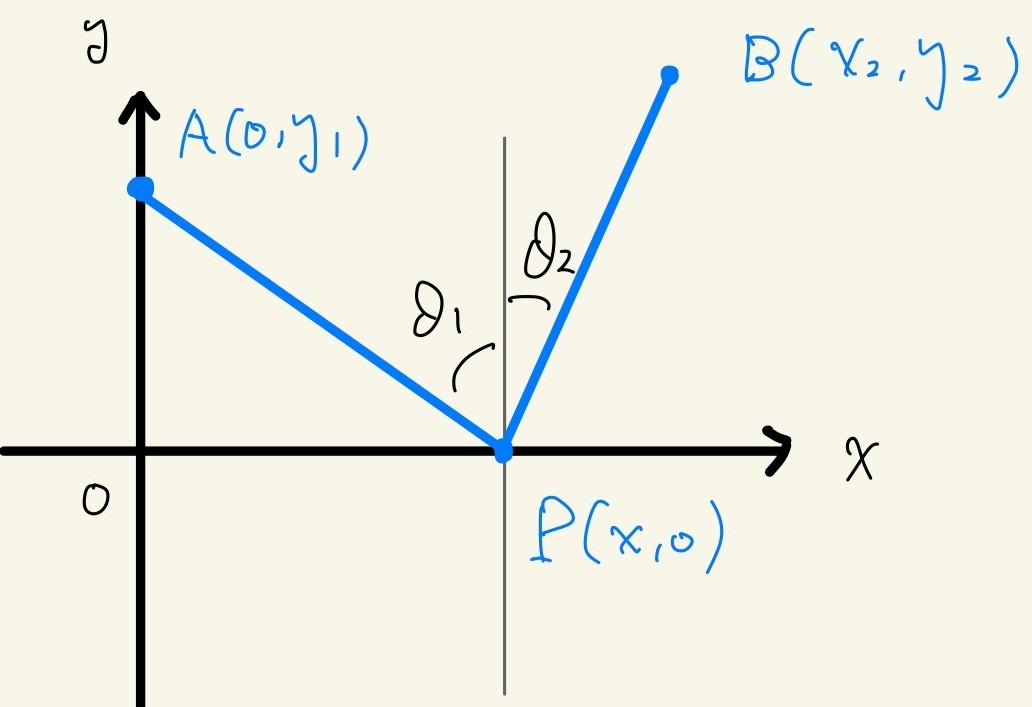
\includegraphics[width=7cm]{ReflectionPrinciple.jpg}
    \end{figure}
\end{exercise}
\begin{proof}
    \[\Om:=\Brace{\gamma:\text{A,Bを結ぶ曲線}\mid\gamma\text{は}x\text{軸と交差する}}.\]
    とおいてFermatの原理を考えるが,$x$軸との交点の1つを$P$とすれば,A$\to$P, P$\to$Bの経路は直線である必要があることは明らか.
    よって,A, P, Bを結ぶ折れ線のみを考えれば十分である.その際の所要時間は,関数
    \[T(x)=\sqrt{x^2+y_1^2}+\sqrt{(x_2-x)^2+y_2^2}\]
    の定数倍になっているから,特に極値点は$T$について調べれば十分.$x\in\R_+$が極値点であるためには,
    \begin{align*}
        T'(x)=\frac{x}{\sqrt{x^2+y_1^2}}-\frac{x_2-x}{\sqrt{(x_2-x)^2+y_2^2}}=\sin\theta_1-\sin\theta_2=0
    \end{align*}
    より,$\theta_1=\theta_2$が必要.
\end{proof}

\begin{exercise}[affine空間上で微分が消えることの特徴付け]
    $A$を(有限次元とは限らない)affine空間,$f:A\to\R$を可微分関数とする.
    次は同値:
    \begin{enumerate}
        \item $df|_a=0$.
        \item 任意の方向$v\in A$について,これを接ベクトルに持つ直線$\varphi(s):=a+sv\;(s\in(-\ep,\ep))$に対して,
        \[D_\varphi f|_a:=\dd{}{s}f(\varphi(s))\biggr|_{s=0}=0.\]
    \end{enumerate}
\end{exercise}
\begin{proof}
    (1)$\Rightarrow$(2)は定義に含意されているから,(2)$\Rightarrow$(1)を示せば良い.
    任意の可微分関数$\psi:(-\ep,\ep)\to A$であって$\psi(0)=a$を満たすものを取ると,ある$v\in A$が一意的に存在して,
    \[\lim_{h\to0}\frac{\psi(h)-(\psi(0)+hv)}{h}=\lim_{h\to0}\frac{\psi(h)-\varphi(h)}{h}=0.\]
    が成り立つ.
    これを$f$の可微分性と併せると,
    \begin{align*}
        \dd{}{s}f(\psi(s))\biggr|_{s=0}&=\lim_{h\to0}\frac{f(\psi(h))-f(a)}{h}\\
        &=\lim_{h\to0}\frac{\Paren{f(\psi(h))-f(\varphi(h))}+\Paren{f(\varphi(h))-f(a)}}{h}\\
        &=0+\dd{}{s}f(\varphi(s))\biggr|_{s=0}=0.
    \end{align*}
\end{proof}

\begin{exercise}[最急降下線の変分法による導出]
    2点の最急降下線はcycloidが与える.すなわち,
    \[\Om:=\Brace{\gamma:[t_0,t_1]\to\R^2\;\middle|\;\begin{array}{l}
    \gamma(t_0)=(0,0),\gamma(t_1)=(a,b).\\
    C^1\text{級の陰関数表示}y:[a,b]\to\R_+\text{を持つ}\\
    \gamma'(t_0)=(0,0).
    \end{array}}\]
    のうち,一様重力場の下で原点からより低い点P$(a,b)$まで最も速く移動する際の運動はcycloid
    \[\gamma(t)=C\vctr{t-\frac{1}{2}\sin 2t}{\frac{1}{2}-\frac{1}{2}\cos 2t},\qquad C>0,t\in[0,t_1],Ct_1-\frac{1}{2}\sin 2t_1=a.\]
    が与える.
\end{exercise}
\begin{proof}\mbox{}
    \begin{enumerate}[{Step}1]
        \item まず,所要時間を表す汎関数$S:\Om\to\R$を求める.
        
        位置$x$での速さを$v(x)$とすると,初期条件$v(0)=0$より,エネルギー保存則から
        \[\frac{1}{2}mv(x)^2=mgy(x)\quad\Leftrightarrow\quad v(x)=\sqrt{2gy(x)}.\]
        位置$x$までの運動の軌跡の長さ$l(x)$は
        \[l(x)=\int^x_0\sqrt{1+y'(x)^2}dx\]
        である.以上から,
        \begin{align*}
            S(\gamma)&=\int^{l(a)}_0\frac{dl}{v(x)}\\
            &=\int^a_0\frac{\sqrt{1+y'(x)^2}}{v(x)}dx=\int^a_0\sqrt{\frac{1+y'(x)^2}{2gy(x)}}dx.
        \end{align*}
        改めて,$S(\gamma)$の$\sqrt{2g}$倍を$S(\gamma)$として取り直しても,極値点は変わらない.
        特に,Lagrangianは
        \[L(y,y'):=\sqrt{\frac{1+y'^2}{y}}.\]
        で与えられる.
        \item 計算
        \[\pp{L}{y}=\frac{1}{2}\paren{\frac{1+y'^2}{y}}^{-\frac{1}{2}}\paren{-\frac{1+y'^2}{y^2}}=-\frac{1}{2}\frac{(1+y'^2)^{\frac{1}{2}}}{y^{\frac{3}{2}}}\]
        \[\pp{L}{y'}=\frac{1}{2}\paren{\frac{1+y'^2}{y}}^{-\frac{1}{2}}2\frac{y'}{y}=\frac{y'}{\sqrt{y(1+y'^2)}}\]
        から,Euler-Lagrange方程式は
        \begin{align*}
            -\frac{1}{2}\frac{(1+y'^2)^{\frac{1}{2}}}{y^{\frac{3}{2}}}&=\dd{}{x}\frac{y'}{\sqrt{y(1+y'^2)}}\\
            &=\frac{y''}{\sqrt{y(1+y'^2)}}+\paren{-\frac{1}{2}}\frac{y'}{\Paren{y(1+y'^2)}^{\frac{3}{2}}}\Paren{(1+y'^2)+2yy'y''}\\
            &=\frac{y''}{\sqrt{y(1+y'^2)}}-\frac{1}{2}\frac{y'}{\sqrt{y^3(1+y'^2)}}-\frac{y'^2y''}{\sqrt{y(1+y'^2)^3}}.
        \end{align*}
        となる.両辺に$\sqrt{y(1+y'^2)}$を乗じることで
        \begin{align*}
            -\frac{1}{2}\frac{1+y'^2}{y}&=y''-\frac{1}{2}\frac{y'}{y}-\frac{y'^2y''}{1+y'^2}\\
            &=\frac{y''}{1+y'^2}-\frac{1}{2}\frac{y'}{y}
        \end{align*}
        より,
        \[-\frac{1}{2y}=\frac{y''}{1+y'^2}\quad\Leftrightarrow y'^2+2yy''+1=0\]
        の形に同値変形出来る.同値性は因子$y(1+y'^2)$が$x=0$の場合を除いて零にならないことによる.
        \item この常備分方程式には積分因子$y'$が見つかり,これを両辺に乗じることで
        \[y'+2yy'y''+y'^3=(y+yy'^2)'=0\]
        を得る.よって,この第一積分を$y+yy'^2=C>0$とおいて解を求める.
        なお,$y\ge 0$として良いから$C\ge0$が必要で,$C=0$のとき$y=0$より$\Om$の元ではない.
        この条件は正規形の常微分方程式
        \[y'=\sqrt{\frac{C-y}{y}}\]
        に帰着するが,これは変数分離型であることに注目すれば,
        \begin{align*}
            x&=\int\sqrt{\frac{y}{C-y}}dy+C'\qquad C'\in\R\\
            &=\int\frac{\sin t}{\cos t}2C\sin t\cos tdt+C'\qquad y=:C\sin^2t\\
            &=C\int(1-\cos 2t)dt+C'\\
            &=C\paren{t-\frac{\sin 2t}{t}}+C'.
        \end{align*}
        と積分出来る.$y=0$のとき$t=0$で,このとき$x=0$が必要だから,$C'=0$を得る.
        総じて,
        \[\begin{cases}
            x=Ct-\frac{C}{2}\sin 2t,\\
            y=C\sin^2t=\frac{C}{2}-\frac{C}{2}\cos 2t.
        \end{cases}\qquad C>0.\]
    \end{enumerate}
\end{proof}

\section{解析力学から幾何学へ}

\subsection{第5回授業:変分原理から見た微分幾何}

\begin{exercise}[停留曲面は極小曲面に同値\footnote{\cite{小林昭七-曲面}問2.4dを参考にした}]
    $R\subset\R^2$を曲面,$C$を$\partial R$の$\R^3$へのある滑らかな埋め込み像とし,
    \[\Om(C):=\Brace{\Sigma\subset\R^3\mid\exists_{\varphi\in C^3(R,\R^3)}\;\varphi(R)=\Sigma,\partial\Sigma=C}.\]
    とし,$S(\Sigma)$をその面積として変分問題$(\Om(C),S)$を定める.このとき,次は同値:
    \begin{enumerate}
        \item $\Sigma$は停留曲面である.
        \item $\Sigma$の平均曲率$H$は消える:$H\equiv0$.
    \end{enumerate}
\end{exercise}
\begin{proof}
    任意の曲面片$\Sigma\in\Om(C)$とそのパラメータ付け$\p(R)=\Sigma$に対して,任意に$f(\partial R)=\{0\}$を満たす可微分関数$f:R\to\R$を取る.
    $\e$を曲面片$\Sigma$上の単位法ベクトル場とし,関数$f$が定める
    曲面$\Sigma$のパラメータ付け$\p$の摂動
    \[\o{\p}:=\p+\ep f\e\qquad(\ep\in\R)\]
    を考え,$\Sigma_\ep:=\o{\p}(R)$で表す.
    補題より,$A(\ep):=S(\Sigma_\ep)$とすると,
    \[A'(0)=-\iint_RfH\,dA=-\iint_RfH\sqrt{g_{11}g_{22}-g_{12}^2}dudv\]
    が成り立つ.
    \begin{description}
        \item[(1)$\Rightarrow$(2)] $\Sigma$が停留曲面であるとき,任意の$f$と$\ep$について$A'(0)=0$が成り立つから,これは変分法の基本補題より,$H\equiv0$を意味する.
        実際,もし$H$がある正の測度を持つ集合上で非零ならば,$\varphi$を$R$内部で正で$\partial R$上で$0$となる関数として,$f$として$\varphi H$を取ると,
        \[A'(0)=-\iint_R\varphi H^2\,dA<0\]
        より矛盾.
        \item[(2)$\Rightarrow$(1)] $H\equiv0$ならば,任意の$f,\ep$について$A'(0)=0$であるから,$\Sigma$は停留曲面である.
    \end{description}
\end{proof}

\begin{lemma*}[曲面の変分に対する面積変化\footnote{\cite{佐々木}4.1節}]
    任意の曲面片$\Sigma\in\Om(C)$とそのパラメータ付け$\p(R)=\Sigma$に対して,任意に$f(\partial R)=\{0\}$を満たす可微分関数$f:R\to\R$を取る.
    $\e$を曲面片$\Sigma$上の単位法ベクトル場とし,関数$f$が定める
    曲面$\Sigma$のパラメータ付け$\p$の摂動
    \[\o{\p}:=\p+\ep f\e\qquad(\ep\in\R)\]
    を考え,$\Sigma_\ep:=\o{\p}(R)$で表す.
    いま,$A(\ep):=S(\Sigma_\ep)$とすると,
    \[A'(0)=-\iint_RfH\,dA=-\iint_RfH\sqrt{g_{11}g_{22}-g_{12}^2}dudv\]
    が成り立つ.
\end{lemma*}
\begin{proof}
    \begin{align*}
        \o{g}_{ij}&:=\o{\p}_i\cdot\o{\p}_j=(\p_i+\ep f_i\e+\ep f\e_i)\cdot(\p_j+\ep f_j\e+\ep f\e_j)\\
        &=g_{ij}+\ep f\e_i\cdot\p_j+\ep^2f_if_j\e\cdot\e+\ep f\e_i\cdot\p_j+(\ep f)^2\e_i\cdot\e_j\\
        &=g_{ij}-2\ep f\cdot h_{ij}+\ep^2(f_if_j+f^2k_{ij}).
    \end{align*}
    最後の等式は,Weingartenの式から$\e_i\cdot\p_j=-h_{ij}$であることによる.
    ただし,$\p_i,f_i,\e_i$は$i=1$のとき
    $u$での偏微分,$i=2$のとき$v$での偏微分とし,
    \[h_{ij}:=\e_i\cdot\p_j,\quad k_{ij}:=\e_i\cdot\e_j.\]
    を第二基本形式の係数と第三基本形式の係数とした.
    以上より,面積要素の変換は,Einsteinの記法に注意して,
    \begin{align*}
        \o{g}_{11}\o{g}_{22}-\o{g}_{12}^2&=\Paren{g_{11}-2\ep fh_{11}+\ep^2(f_1^2+f^2k_{11})}\Paren{g_{22}+2\ep fh_{22}+\ep^2(f^2_2+f^2k_{22})}\\
        &\qquad\qquad-\Paren{g_{12}+2\ep f_{12}+\ep^2(f_1f_2+f^2k_{12})}^2\\
        &=(g_{11}g_{22}-g_{12}^2)\Biggl(1 - 2\ep f\underbrace{\frac{h_{11}g_{22}+g_{11}h_{22}-2h_{12}g_{12}}{\abs{g_{ij}}}}_{=g^{ij}h_{ij}=2H} +4 \ep^2f^2\underbrace{\frac{\abs{h_{ij}}}{\abs{g_{ij}}}}_{=K}\\
        &\qquad\qquad+\ep^2f^2\underbrace{\frac{g_{11}k_{22}+g_{22}k_{11}-g_{12}k_{12}-g_{21}k_{21}}{\abs{g_{ij}}}}_{=g^{ij}k_{ij}}+\ep^2\frac{f_1^2g_{22}+f_2^fg_{11}-2f_1f_2g_{12}}{\abs{g_{ij}}}\Biggr)+o(\ep^3)\\
        &=(g_{11}g_{22}-g_{12}^2)\Paren{1-4\ep fH+\ep^2f^2(4K+g^{ij}k_{ij}+g^{ij}f_if_j)}+o(\ep^3)
    \end{align*}
    と変換される.
    ただし,$\abs{g_{ij}}$は行列$\mtrx{g_{11}}{g_{12}}{g_{21}}{g_{22}}$の行列式,$K$はGauss曲率とした.
    この計算から,ある$c>0$が存在して,任意の十分に小さい$\ep>0$について,
    \[\Abs{\sqrt{\o{g}_{11}\o{g}_{22}-\o{g}_{12}^2}-\sqrt{g_{11}g_{22}-g_{12}^2}(1-2\ep fH)}<c\ep^2\]
    すなわち,
    \[\Abs{A(\ep)-A(0)+2\ep\iint_RfHdA}<c'\ep^2\]
    \[\Abs{\frac{A(\ep)-A(0)}{\ep}+2\iint_RfH\,dA}<c'\ep.\]
    以上より,
    \[A'(0)=-2\iint_RfH^,dA\]
    を得た.
\end{proof}

\begin{exercise}[中心力場の特徴付け]
    任意の有界な軌道が閉曲線になる中心力場は,次の2つに限る:
    \begin{enumerate}
        \item Kepler問題:$U=-\frac{\kappa}{r}\;(\kappa>0)$.
        \item 調和振動子:$U=\frac{a}{2}r^2\;(a>0)$.
    \end{enumerate}
\end{exercise}

\subsection{第6回授業:Gauge固定とエネルギー汎関数}

\begin{exercise}[長さ汎関数のgauge変換不変性]
    $M$をRiemann多様体,$\gamma:[a,b]\to M$を
    可微分曲線,
    $f:[c,d]\iso[a,b]$を$f(a)=c,f(d)=b$を満たす可微分同相とする.
    このとき,
    \[\L(\gamma)=\L(\gamma\circ f).\]
\end{exercise}
\begin{proof}
    \[G:=\mtrx{g_{11}}{g_{12}}{g_{21}}{g_{22}}\]
    をRiemann計量の係数行列,$\wgamma:=\gamma\circ f$とすると,
    \begin{align*}
        \L(\gamma\circ f)&=\int^d_c\sqrt{(\wt{\gamma}'|G\circ\wgamma\cdot\wt{\gamma}')}ds\\
        &=\int^d_c\sqrt{(\gamma'(f(s))f'(s)|G\circ\wgamma\cdot\gamma'(f(s))f'(s))}ds\\
        &=\int^d_c\sqrt{(\gamma'(f(s))|G(\gamma(f(s)))\cdot\gamma'(f(s)))}f'(s)ds\\
        &=\int^b_a\sqrt{(\gamma'(t)|G(\gamma(t))\cdot\gamma'(t))}dt=\L(\gamma).
    \end{align*}
    ただし,$(-|-)$は各点$\gamma(t)$での接空間の内積とした.
\end{proof}

\begin{exercise}[affineパラメータへの取替]
    任意の微分が消えない曲線$\gamma:[a,b]\to M$に対して,パラメータの変換$f:[c,d]\to[a,b]$であって,
    $\gamma\circ f$がaffineパラメータになるようなものが存在する.
\end{exercise}
\begin{proof}
    $c:=0,d:=L(\gamma)$とし,
    $\varphi:[a,b]\to[c,d]$を
    \[\varphi(t):=\int^{t}_a\norm{\gamma'(t)}dt\]
    と定めると,$\varphi'(t)=\norm{\gamma'(t)}\;(t\in[a,b])$が成り立つ.
    $\gamma$は正則としたから$\varphi'>0$
    より狭義単調増加であり,
    特に可微分同相である.よって,可微分な逆$\varphi^{-1}$を持つから,これについて$\wgamma:=\gamma(\psi)$とすれば良い.
    実際,
    \[\wgamma'(s)=\gamma'(\psi(s))\psi'(s)=\frac{\gamma'(\psi(s))}{\norm{\gamma'(\psi(s))}}\qquad(s\in[c,d]).\]
    より,これは弧長が定めるパラメータである.
\end{proof}

\begin{exercise}[正規座標系の定義\footnote{\cite{Petersen16-RiemannianGeometry}命題5.5.1}]
    $n$次元
    Riemann多様体$M^n$の任意の点$x\in M$について,
    $(x,v)\in T(M)$を$t=0$に通る測地線$c_v:(-\ep,\ep)\to M$は唯一つに定まる.
    このとき,接空間内のある開集合$U\osub T_x(M)$が存在して,
    \[\xymatrix@R-2pc{
        \exp_x:U\subset T_x(M)\ar[r]&M\\
        \rotatebox[origin=c]{90}{$\in$}&\rotatebox[origin=c]{90}{$\in$}\\
        v\ar@{|->}[r]&c_v(1)
    }\]
    は$x\in M$の近傍座標を与える.
\end{exercise}
\begin{proof}\mbox{}
    \begin{description}
        \item[方針] \[O_x:=\Brace{v\in T_x(M)\mid v\text{を初速度とする測地線}c_v\text{は}[0,1]\text{の近傍で定まる}}.\]
        とすると,$0\in O_x$である.写像$\exp_x:O_x\to M$の微分の$0\in T_x(M)$での値
        \[d\exp_x:T_0(T_x(M))\to T_x(M)\]
        が非特異であることを示せば良い.
        すると,逆関数定理から$\exp_x$は局所微分同相であるから,$0\in T_x(M)$のある開近傍$U\osub T_x(M)$が存在して$\exp_x|_U$は可微分同相であり,
        $x\in\exp_x(U)$である.
        \item[準備] 任意の$\al>0$と,$c_{\al v}$の定義されている任意の$t\in\R_+$について,$c_{\al v}(t)=c_v(\al t)$が成り立つ.
        実際,$t\mapsto c_v(\al t)$は$t=0$にて$(x,\al v)$を通る$T(M)$上の曲線であるが,常微分方程式系の初期値問題の解の一意性から,これは$c_{\al v}$に等しい.
        \item[証明] よって,$O_x$の定め方から,任意の$v\in O_x$について$c_v(t)=c_{tv}(1)\;(t\in[0,1])$が成り立つ.さらに,
        \[I_0(v):=\dd{}{t}(tv)\biggr|_{t=0},\qquad(v\in T_p(M)).\]
        により定まる線型写像$T_p(M)\to T_0(T_p(M))$は同型である.これは$T_p(M)$の局所自明性から明らか.
        いま,
        \begin{align*}
            d\exp_x(I_0(v))&=\dd{}{t}\exp_x(tv)\biggr|_{t_0}&\text{写像の微分の定義}\\
            &=\dd{}{t}c_{tv}(1)\biggr|_{t_0}&\text{指数写像の定義}\\
            &=\dd{}{t}c_v(t)\biggr|_{t=0}=v.
        \end{align*}
        より,$d\exp_x\circ I_0=\id_{T_p(M)}$を得る.特に,$T_0(T_p(M))$の原点にて非特異である.
    \end{description}
\end{proof}

\subsection{第7回授業:Lie群の測地線}

\begin{exercise}[指数写像と行列の指数関数]
    Lie群$G\subset\GL_n(\C)$の測地線は$\gamma(t)=\gamma(0)e^{tX}$の形で与えられる.
\end{exercise}

\begin{exercise}[de Sitter空間の例]
    $\SL_2(\R)$のLie環は
    \[\r{sl}_2(\R):=\Brace{A\in M_2(\R)\mid\tr(A)=0}.\]
    なる3次元空間になる.一般に
    $\det(e^A)=e^{\tr(A)}$が成り立つことに注意.このとき,
    指数写像$\exp:\r{sl}_2(\R)\to\SL_2(\R)$は全射でない.
\end{exercise}
\begin{proof}
    $g\in\SL_2(\R)$であって,$\tr g<-2$を満たすものを取れば,
    これは$e^X\;(X\in \SL_2(\R))$の形では表せない.例えば
    \[g=\mtrx{-2}{0}{0}{-\frac{1}{2}}\]
    など.
    
    任意に$X\in \SL_2(\R)$を取り,その固有値を$\al,\beta$とすると,
    \[\tr(e^X)=e^\al+e^\beta\]
    が成り立つことはすぐに分かる.
    $\al,\beta$がいずれも実数である場合は,これは$0$より大きい.
    $\al,\beta$が実数でない場合は,ある$a,b\in\R$を用いて$\{\al,\beta\}=\{a\pm bi\}$と表せるが,
    $\tr(X)=0$より$a=0$が必要.
    よって,
    \[\tr(e^X)=e^{bi}+e^{-bi}=2\cos b\ge-2.\]
    いずれの場合も,$\tr(g)=\tr(e^X)<-2$としたことに矛盾.
\end{proof}

\subsection{第8回授業:Legendre変換の応用}

\begin{theorem*}[Minkowski内積の双曲角による表示\footnote{\cite{Callahan00-Spacetime}Th'm 2.8}]
    任意の未来方向の時間的事象$\r{E_1,E_2}$について,
    その双曲角を$\angle\r{E_1E_2}=:\beta$とすると,
    \[\rE_1\cdot\rE_2=\norm{\rE_1}\norm{\rE_2}\cosh\beta.\]
\end{theorem*}
\begin{proof}
    Minkowski空間を$\R^2$として考える.一般の場合も,空間変数$z$を多次元に解釈し,
    $z^2=\sum_{i\in[n]}z_i^2$と読み替えることで
    同様に示せる.
    \begin{enumerate}[{Step}1]
        \item 単位化を$\rU_i:=\frac{\rE_i}{\norm{\rE_i}}\;(i=1,2)$とすると,これは標準双曲線上の点である.
        Lorentz変換は双曲角を保つから,
        ある$u\in\R$が存在して,
        \[H_u(\rU_1)=\vctr{1}{0},\quad H_u(\rU_2)=\vctr{\cosh\beta}{\sinh\beta}.\]
        と表せる.これについて,
        \[H_u(\rU_1)\cdot H_u(\rU_2)=(1\;0)\mtrx{1}{0}{0}{-1}\vctr{\cosh\beta}{\sinh\beta}=\cosh\beta\]
        がわかり,Lorentz変換はMinkowski内積を保つから,$\rU_1\cdot \rU_2=H_u(\rU_1)\cdot H_u(\rU_2)=\cosh\beta$である.
        \item 元のベクトルについても,Minkowski内積の双線型性から,
        \[\rE_1\cdot\rE_2=(\norm{\rE_1}\rU_1)\cdot(\norm{\rE_2}\rU_2)=\norm{\rE_1\rE_2}(\rU_1\cdot \rU_2)=\norm{\rE_1\rE_2}\cosh\beta.\]
    \end{enumerate}
\end{proof}

\begin{exercise}[Minkowski空間に於ける逆向きの三角不等式]
    任意の未来方向の時間的事象$\r{E_1,E_2}$について,$\angle\r{E_1E_2}=:\beta$とする.
    \begin{enumerate}
        \item $\norm{\r{E_1+E_2}}^2=\norm{\r{E_1}}^2+\norm{\r{E_2}}^2+2\norm{\r{E_1}}\norm{\r{E_2}}$.
        \item 逆向きの三角不等式:$\norm{\r{E_1+E_2}}^2\ge\norm{\r{E_1}}+\norm{\r{E_2}}$.
    \end{enumerate}
\end{exercise}
\begin{proof}\mbox{}
    \begin{enumerate}
        \item $\rE_1+\rE_2$は再び未来方向かつ時間的事象である.実際,
        \[\rE_1=\vctr{t_1}{z_1},\quad\rE_2=\vctr{t_2}{z_2}\]
        とすると,$-(t_1+t_2)<z_1+z_2<t_1+t_2$であることが解る.
        これについて,
        \begin{align*}
            \norm{\rE_1+\rE_2}^2&=(\rE_1+\rE_2)\cdot(\rE_1+\rE_2)=\norm{\rE_1}^2+\norm{\rE_2}^2+2\rE_1\cdot\rE_2\\
            &=\norm{\rE_1}^2+\norm{\rE_2}^2+2\norm{\rE_1}\norm{\rE_2}\cosh\beta.
        \end{align*}
        \item $\cosh\beta=\frac{e^\beta+e^{-\beta}}{2}\ge\sqrt{e^\beta\cdot e^{-\beta}}=1$より,(1)から
        \begin{align*}
            \norm{\rE_1+\rE_2}&=\sqrt{\norm{\rE_1}^2+\norm{\rE_2}^2+2\norm{\rE_1}\norm{\rE_2}\cosh\beta}\\
            &\ge\sqrt{\norm{\rE_1}^2+\norm{\rE_2}^2+2\norm{\rE_1}\norm{\rE_2}}=\norm{\rE_1}+\norm{\rE_2}.
        \end{align*}
    \end{enumerate}
\end{proof}

\section{解析力学再論}

\subsection{第9回授業:Hamiltonの変分原理}

\begin{lemma*}[逆行列の微分則]
    可微分写像$x\mapsto A(x)\in\GL_n(\C)$について,
    \[(A^{-1})'=-A^{-1}A'A^{-1}\]
\end{lemma*}
\begin{proof}
    等式$AA^{-1}=I$の両辺を微分すると,
    \[A'A^{-1}+A(A^{-1})'=O\]
    より従う.
\end{proof}

\begin{exercise}[測地流の方程式のHamilton系としての特徴付け]
    Riemann多様体上の曲線について,次の2条件は同値:
    \begin{enumerate}
        \item Lagrange形式:弧長の定めるパラメータ$s$について,
        \[\dd{^2\gamma^m}{t^2}+\Gamma_{kl}^i\dd{\gamma^k}{s}\dd{\gamma^l}{s}=0,\qquad(m\in[n]).\]
        \item Hamilton形式:次の方程式を満たす
        \[\begin{cases}
            \dd{x^m}{t}=g^{mi}p_i,\\
            \dd{p^i}{t}=-\frac{1}{2}\pp{g^{lk}}{x^i}p_lp_k.
        \end{cases}\]
    \end{enumerate}
\end{exercise}
\begin{proof}
    (2)の2式を併せると,
    \begin{align*}
        \dd{^2x^m}{t^2}&=g^{mi}\dd{p^i}{t}\\
        &=g^{mi}\paren{-\frac{1}{2}\pp{g^{lk}}{x^i}p_lp_k}.
    \end{align*}
    を得る.さらに(2)の第1式は
    \[p_l=(g^{kl})^{-1}\dd{x^k}{t}\]
    に同値で,これを代入することで,
    \begin{align*}
        \dd{^2x^m}{t^2}&=\frac{1}{2}g^{mi}\paren{-\pp{g^{lk}}{x^i}(g^{kl})^{-1}(g^{lk})^{-1}}\dd{x^k}{t}\dd{x^l}{t}\\
        &=\frac{1}{2}g^{mi}\pp{g_{kl}}{x^i}\dd{x^k}{t}\dd{x^l}{t}.
    \end{align*}
    と計算を進められる.ただし,途中で逆行列の微分$(A^{-1})'=-A^{-1}A'A^{-1}$を用いた.
    最後に,$t$の代わりに弧長の定めるパラメータ$s$に取り替えることを考えると,
    \[\frac{1}{2}\pp{g_{kl}}{x^i}\dd{x^k}{t}\dd{x^l}{t}=-\Gamma^{i}_{kl}\dd{x^k}{s}\dd{x^l}{s}\dd{s}{t}\]
    以上を併せると,
    \[\paren{\dd{^2\gamma^m}{t^2}+\Gamma_{kl}^i\dd{\gamma^k}{s}\dd{\gamma^l}{s}}\dd{s}{t}=0\]
    いま$t$は正則なパラメータと考えて良いから,$\dd{s}{t}\ne0$より,結論を得る(以上の変形はいずれも逆に辿れる同値変形である).
\end{proof}

\subsection{第10回授業:Noetherの定理}

\begin{exercise}[ベクトル場の方向微分としての特徴付け\footnote{\cite{志賀浩二-多様体}定理3.2}]
    $n$次元可微分多様体$M^n$について,
    \[\Der(C^\infty(M)):=\Brace{D\in\End(C(M))\mid\forall_{f,g\in C^\infty(M)} D(fg)=fD(g)+gD(f)}.\]
    とすると,$\Der(C^\infty(M))\simeq_\Set\X(M)$である.
\end{exercise}
\begin{proof}\mbox{}
    \begin{description}
        \item[$\supset$] 任意のベクトル場$X\in\X(M)$を取ると,任意の点$x\in M$で$X_x(fg)=(X_xf)g(x)+f(x)X_xg$を満たす.
        \item[$\subset$] 
        \begin{description}
            \item[問題の所在] 任意に$D\in\Der(C^\infty(M))$を取る.任意の点$x\in M$において,対応$f\mapsto D(f)(x)$はLeibniz則を満たす線型変換だから,
            ある接ベクトル$X_x\in T_x(M)$が存在して,
            \[X_x(f)=D(f)(x)\]
            を満たす.あとは,この対応$x\mapsto X_x$が接束$T(M)$の滑らかな切断を定めることを示せば良い.
            \item[証明] 任意の$x\in M$とその近傍座標$U$を取り,係数を
            \[X_x=\sum_{\mu=1}^nX^\mu(x)\pp{}{x^\mu}.\]
            とおくと,各係数$X^\mu$は$U$上で滑らかである.実際,$U$上で座標関数$x^\mu$に一致するような,$M$上への滑らかな延長$f\in C^\infty(M)$を取ると,$D(f)\in C^\infty(M)$であるから,
            \[D(f)(x)=X_x(f)=X^\mu(x)\qquad(x\in U).\]
            より$X^\mu\in C^\infty(U)$が従う.

            同様の条件を満たすベクトル場は$X$と同じ係数を持つ必要があるから,存在と一意性が判った.
        \end{description}
    \end{description}
\end{proof}

\section{Symplectic幾何学}

\subsection{第11回授業:Symplectic幾何学}

\begin{exercise}[symplectic空間が定める複素内積空間]
    任意の$2n$次元symplectic線型空間$(V,\om)$に対して,
    ある複素構造$J^2=-\id_V$が存在して,
    $g(x,y):=\om(x,Jy)$について,
    $(V,J)$は$n$次元複素内積空間となる.
\end{exercise}
\begin{proof}\mbox{}
    \begin{description}
        \item[複素線型空間として$V$を見る] $V$の標準基底$\al_1,\cdots,\al_n,\beta_1,\cdots,\beta_n$を取ると,これについて$\om$の行列表示は
        $J_n:=\mtrx{O_n}{I_n}{-I_n}{O_n}$となる.
        これを用いて,複素構造$J:V\to V$を$-J_n$倍線型写像とする.
        このとき,$J(\al_i)=-J_n\al_i=\beta_i$に注意すれば,作用
        \[\xymatrix@R-2pc{
            \rho:\C\times V\ar[r]&V\\
            \rotatebox[origin=c]{90}{$\in$}&\rotatebox[origin=c]{90}{$\in$}\\
            (\xi+i\eta,x)\ar@{|->}[r]&\xi x+\eta J(x)
        }\]
        の$\al_i$-軌道は$\brac{\al_i,\beta_i}$という形の部分空間となる.
        よって,$V$は上記の$\rho$をスカラー倍とすることで,
        $\al_1,\cdots,\al_n$を基底とする$n$次元複素線型空間とみなせる.
        これを$V'$と表す.
        \item[$g$が内積となる] 
        \[g(x,y):=\om(x,Jy)\]
        と定めると,$g$は$V'$の内積である.
        実際,その$\al_1,\cdots,\al_n$に関する行列表示は
        \[g(\al_i,\al_j)=\om(\al_i,J\al_j)=\om(\al_i,\beta_j)=\delta_{ij}.\]
        より,$g$は確かに半正定値な対称形式である.
        半線形性は,第一引数に関する線形性は明らかで,第二引数についても,任意の$x,y\in V$と$z\in\C$について,
        \[g(x,(\xi+i\eta)y)=\om(x,J(\xi+i\eta)y)=\om(x,J\xi y)+\om(x,J^2\eta y)=\om\]
        非退化性も明らかである.
    \end{description}
\end{proof}

\begin{exercise}
    $(V^{2n},\om)$をsymplectic部分空間,$W,W_1,W_2\subset V$を線型部分空間とする.
    \begin{enumerate}
        \item $\dim W+\dim W^\perp=\dim V$.
        \item $(W^\perp)^\perp=W$.
        \item $W_1\subset W_2\Leftrightarrow W_1^\perp\supset W_2^\perp$.
        \item $(W_1+W_2)^\perp=W_1^\perp\cap W_2^\perp$.
        \item $(W_1\cap W_2)^\perp=W_1^\perp+W_2^\perp$.
    \end{enumerate}
\end{exercise}
\begin{proof}
    $V$のsymplectic基底を$e_1,\cdots,e_{2n}$とすると,これについて$\om$は行列$J_n:=\mtrx{O_n}{I_n}{-I_n}{O_n}$によって表現される.
    \begin{enumerate}
        \item $\om^\#:V\to V^*$の誘導する線型写像
        \[\xymatrix@R-2pc{
            f:V\ar[r]&W^*\\
            \rotatebox[origin=c]{90}{$\in$}&\rotatebox[origin=c]{90}{$\in$}\\
            x\ar@{|->}[r]&\om(x,-)|_{W}
        }\]
        を考えると,$\Ker f=W^\perp$である.
        またこの線型写像は全射であることは,$\om^\#$と全射$i^*:V^*\epi W^*$の合成であることによる.
        よって,$\dim V=\dim W+\dim W^\perp$.
        \item \begin{description}
            \item[$W\subset(W^\perp)^\perp$] $(W^\perp)^\perp$の元であるための必要十分条件は,$\forall_{y\in W^\perp}\;\om(x,y)=0$を満たすことであるが,
            そもそも任意の$y\in W^\perp$は任意の$x\in W$に対して$\om(x,y)=0$を満たすから,任意の$x\in W$は$(W^\perp)^\perp$の元である.
            \item[$W=(W^\perp)^\perp$] 
            (1)から
            \[\dim W+\dim W^\perp=\dim V=\dim W^\perp+\dim (W^\perp)^\perp\]
            より,$\dim W=\dim(W^\perp)^\perp$.よって特に等号が成り立つことがわかる.
        \end{description}
        \item 
        \begin{description}
            \item[$\Rightarrow$] $x\in W_2^\perp$を任意にとる.
            すると$\forall_{y\in W_2}\;\om(y,x)=0$であるから,特に$x\in W^\perp_1$.
            \item[$\Leftarrow$] $\Rightarrow$の結果と(2)から
            \[W_1=(W_1^\perp)^\perp\subset(W_2^\perp)^\perp=W_2.\]
        \end{description}
    \end{enumerate}
    \begin{description}
        \item[(4),(5)] \mbox{}
        \begin{enumerate}[{Step}1]
            \item 任意の$x+y\in W_1^\perp+W_2^\perp$を取ると,
            \[\forall_{z\in W_1\cap W_2}\;\om(x+y,z)=\om(x,z)+\om(y,z)=0.\]
            であるから,$x+y\in(W_1\cap W_2)^\perp$.
            これより$W_1^\perp+W_2^\perp\subset(W_1\cap W_2)^\perp$である.
            両辺の直交を取ると$(W_1^\perp+W_2^\perp)^\perp\subset W_1\cap W_2$であるが,
            $W_1,W_2$をその直交に取り直すことで$(W_1+W_2)^\perp\subset W_1^\perp\cap W_2^\perp$も成り立つ.
            \item 任意の$x\in(W_1+W_2)^\perp$を取ると,
            \[\forall_{y\in W_1}\;\forall_{z\in W_2}\;\om(x,y+z)=\om(x,y)+\om(x,z)=0.\]
            が成り立つ.特に$y=0,z=0$の場合をそれぞれ考えると,$x\in W_1^\perp$かつ$x\in W_2^\perp$であることがわかるから,
            $(W_1+W_2)^\perp\subset W_1^\perp\cap W_2^\perp$.
            両辺の直交を取ると$(W^\perp_1\cap W^\perp_2)^\perp\subset W_1+W_2$であり,
            $W_1,W_2$をその直交に取り直すことで$(W_1\cap W_2)^\perp\subset W_1^\perp+W_2^\perp$.
        \end{enumerate}
    \end{description}
\end{proof}

\begin{exercise}
    $\dim V=2n$,$W\subset V$を線型部分空間とする.
    \begin{enumerate}
        \item $W$がisotropicならば,$\dim W\le n$.
        \item $W$がcoisotropicならば,$\dim W\ge n$.
    \end{enumerate}
    特に,$W$がLagrangeならば,$\dim W=n$である.
\end{exercise}
\begin{proof}\mbox{}
    \begin{enumerate}
        \item $W$がisotropicとは,$W\subset W^\perp$ということである.このとき当然$\dim W\le\dim W^\perp$.
        いま,等式$\dim W+\dim W^\perp=2n$より,$2\dim W\le\dim W+\dim W^\perp=2n$.
        \item $W$がcoisotropicのとき,$W^\perp$はisotropicであるから,(1)より$\dim W^\perp\le n$.よって,$\dim W\ge n$.
    \end{enumerate}
\end{proof}

\subsection{第12回授業:Symplectic多様体}

\begin{exercise}
    $A$をsymplectic空間$(V,\om)$の自己準同型とする.
    $\det A=1$である.
\end{exercise}
\begin{proof}
    $A$が定める線型写像$f_A:V\to V$の外積
    \[\Lambda^2f_A:\Lambda^2V\to\Lambda^2V\]
    について,symplectic形式は交代形式だから,次の図式は可換になる:
    \[\xymatrix{
        \Lambda^2V\ar[dr]_-\om\ar[rr]^-{\Lambda^2f_A}&&\Lambda^2V\ar[dl]^-\om\\
        &\R
    }\]
    一方で,$p=\dim V$の場合,$\Lambda^pf_A$とは$\det A$倍写像になる.
    この2点と$\Lambda^{2n}V=\Lambda^n(\Lambda^2V)$に注意すれば,
    次の図式の大外周りを見比べることで,$\det f_A=1$.
    \[\xymatrix{
        \R\ar[r]^-1&\R\\
        \Lambda^n(\Lambda^2V)\ar[r]^-{\Lambda^n(\Lambda^2f_A)}\ar[u]^-\om\ar@{=}[d]&\Lambda^n(\Lambda^2V)\ar[u]_-\om\ar@{=}[d]\\
        \Lambda^{2n}V\ar[r]^-{\Lambda^{2n}f_A}\ar@{=}[d]&\Lambda^{2n}V\ar@{=}[d]\\
        \R\ar[r]_-{\det A}&\R
    }\]
\end{proof}



\subsection{第13回授業:Arnold-Liouvilleの定理}

\begin{exercise}
    $f$をHamiltonianとする$M$上のベクトル場を$X_f$とする.このとき,任意の$Y\in\X(M)$に対して,
    \[\om(Y,X_f)=(df|Y).\]
    が成り立つ.
\end{exercise}
\begin{proof}
    任意の点$p\in M$について,
    近傍座標$p_1,\cdots,p_n,q_1,\cdots,q_n$であってこれについて$\om$が
    \[\om=\sum_{i\in[n]}dp_i\wedge dq_i\]
    と表せるものを取ると,
    \begin{align*}
        \om_p(Y,X_f)&=\sum_{i\in[n]}(dp_i\wedge dq^i)(Y,X_f)\\
        &=\sum_{i\in[n]}\paren{\pp{f}{p_i}dp_i\wedge dq^i\paren{Y,\pp{}{q_i}-\pp{f}{q_i}dp_i\wedge dq_i\paren{Y,\pp{}{p_i}}}}\\
        &=\sum_{i\in[n]}\paren{\pp{f}{p_i}dp_i(Y)+\pp{f}{q^i}dq^i(Y)}=(df|Y).
    \end{align*}
    と各点$p\in M$上で計算できる.
\end{proof}

\bibliography{../../StatisticalSciences.bib,../../SocialSciences.bib,../../mathematics.bib,../../statistics.bib}

\end{document}

\begin{exercise}
    $A\in\Sp(V,\om)$の固有多項式$\Phi_A$は相反多項式(reciprocal polynomial)である.
\end{exercise}

\begin{exercise}[三すくみの関係]
    \begin{align*}
        \rO_{2n}(\R)\cap\Sp_{2n}(\R)&=\Sp_{2n}(\R)\cap\GL_n(\C)\\
        &=\GL_n(\C)\cap\rO_{2n}(\R)\\
        &=U_n(\C)
    \end{align*}
\end{exercise}

\begin{exercise}[Liouvilleの1-形式の同値な定義]
    $\theta\in\Om^1(M)$について,次の2条件は同値:
    \begin{enumerate}
        \item $\theta=p_1dq^1+\cdots+p_ndq^n$と表せる.
        \item 余接束$\pi:T^*(M)\to M$が引き起こす線型写像$\pi_*:T(T^*(M))\to T(M)$について,$\theta(\xi):=(y|\pi_*\xi)\;(y\in T_x^*(M),\xi\in T_y(T^*(M)))$が成り立つ.
    \end{enumerate}
\end{exercise}